\documentclass[12pt]{report}
\setcounter{secnumdepth}{5}
% includes
\usepackage{geometry}           % page size
\usepackage[utf8]{inputenc}     % encoding

\usepackage{palatino} 

\usepackage[spanish,mexico]{babel}    % language
\usepackage{graphicx}           % images
\usepackage{indentfirst}        % indentation
\usepackage[nottoc]{tocbibind}  % table of contents style
\usepackage[unicode]{hyperref}  % references from the table of contents
\usepackage{adjustbox} %para ajustar las tablas
\usepackage{afterpage} %para paginas en blanco
\usepackage{algorithm}
\usepackage{algpseudocode}  % para pseudocodigo
\floatname{algorithm}{Algoritmo}
\renewcommand{\listalgorithmname}{Lista de algoritmos}
\renewcommand{\algorithmicrequire}{\textbf{Entrada:}}
\renewcommand{\algorithmicensure}{\textbf{Salida:}}
\renewcommand{\algorithmicend}{\textbf{fin}}
\renewcommand{\algorithmicif}{\textbf{si}}
\renewcommand{\algorithmicthen}{\textbf{entonces}}
\renewcommand{\algorithmicelse}{\textbf{si no}}
\renewcommand{\algorithmicfor}{\textbf{para}}
\renewcommand{\algorithmicforall}{\textbf{para todo}}
\renewcommand{\algorithmicdo}{\textbf{hacer}}
\renewcommand{\algorithmicwhile}{\textbf{mientras}}
\renewcommand{\algorithmicloop}{\textbf{repetir}}
\renewcommand{\algorithmicrepeat}{\textbf{repetir}}
\renewcommand{\algorithmicuntil}{\textbf{hasta que}}

\renewcommand{\algorithmicreturn}{\textbf{devolver}} 

 % mi archivo de traducción
\usepackage{enumitem}% http://ctan.org/pkg/enumitem
\usepackage{xcolor}

% black mode
%\usepackage[sfdefault]{roboto} % font
%\pagecolor[rgb]{0.1058823529411765, 0.1294117647058824, 0.1725490196078431} 
%\color[rgb]{0.95,0.95,0.95}
% end black mode

\newcommand\blankpage{% para afterpage
    \null
    \thispagestyle{empty}%
    \addtocounter{page}{-1}%
    \newpage}
    
% includes options
\geometry{  a4paper,            % scientific thesis standard
            left=3cm,
            right=2cm,
            top=2cm,
            bottom=2cm,
 }
\graphicspath{{images/}}        % path where the images are located
\setlength{\parindent}{1cm}     % paragraph indentation

% other options
\linespread{1.5}                % space between lines
\renewcommand*\contentsname{Contenido}    % table of contents name

% the document content
\begin{document}
    % macros (global)
    \newcommand{\university}    {Universidad Nacional de la Pampa}
\newcommand{\universityg}   {Universidad Nacional de la Pampa} % genitive
\newcommand{\faculty}       {Facultad de Ingeniería}
\newcommand{\facultyg}      {Facultad de Ingeniería} % genitive
\newcommand{\speciality}    {sistemas}
\newcommand{\promotion}     {2019}                                  %<---------

\newcommand{\thesistype}    {Plan de trabajo correspondiente a la tesis en ingeniería en sistemas}
\newcommand{\thesistitle}   {Un algoritmo de evolución diferencial híbrido para resolver el problema de planificación de tareas flexible}    %<---------

\newcommand{\authorlast}    {Morero}                               %<---------
\newcommand{\authorfirst}   {Franco Marcelo}
\newcommand{\authornamefl}  {\authorfirst \space \authorlast} % first name first
\newcommand{\authornamelf}  {\authorlast \space \authorfirst} % last name first
\newcommand{\authorbirth}   {03 septiembre 2019}                      %<---------
\newcommand{\authoraddress} {General Pico, La Pampa, Argentina} %<---------
\newcommand{\authorcnp}     {1234567891234}                         %<---------

\newcommand{\session}       {abril, 2020}                       %<---------
\newcommand{\coordinator}   {Dra. Salto Carolina}               %<---------

\newcommand{\dottedline}    {............................}
    
    % front-matter
    \pagenumbering{gobble}
    
    % define the cover page
\begin{titlepage}
    \begin{center}
        % the university and faculty
        \large
        \MakeUppercase{\university}
        
        \LARGE
        \textbf{\MakeUppercase{\faculty}}
        
        % the faculty logo
        \vspace{1cm}
        
\includegraphics[width=0.3\textwidth]{logoFacu.png}
        
        % thesis title
        \vspace{1cm}
        \Large
        \MakeUppercase{\thesistype}
        
        \vspace{0.5cm}
        \LARGE
        \textbf{\thesistitle}
        
        % author
        \vspace{2cm}
        \Large
        Autor
        
        \vspace{0.5cm}
        \LARGE
        \textbf{\authornamefl}
        
        % session
        \vfill
        \Large
        \textbf{Fecha:} \session
        
        % scientific coordinator
        \vspace{2cm}
        \Large
        Director
        
        \vspace{0.5cm}
        \LARGE
        \textbf{\coordinator}
    \end{center}
\end{titlepage}
    % % define the title page
\begin{titlepage}
    \begin{center}
        % the university and faculty
        \large
        \MakeUppercase{\university}
        
        \LARGE
        \textbf{\MakeUppercase{\faculty}}
        
        % thesis title
        \vspace{8cm}
        \huge
        \textbf{\thesistitle}
        
        % author
        \vspace{2cm}
        \LARGE
        \textbf{\authornamefl}
        
        % session
        \vfill
        \Large
        \textbf{Fecha:} \session
        
        % scientific coordinator
        \vspace{4cm}
        \Large
        Director
        
        \vspace{0.5cm}
        \LARGE
        \textbf{\coordinator}
    \end{center}
\end{titlepage}
    %  \vspace*{\fill}

\begin{flushright}
    Avizat, \\
    Îndrumător lucrare de licență, \\
    \coordinator. \\
    Data: \dottedline \hspace{1cm} Semnătura: \dottedline
\end{flushright}

\vspace{1cm}
\begin{center}
    \large
    \textbf{Declarație privind originalitatea conținutului lucrării de licență}
\end{center}

Subsemnatul \textbf{\authornamelf} domiciliat în \textbf{\authoraddress}, născut la data de \textbf{\authorbirth}, identificat prin CNP \textbf{\authorcnp}, absolvent al \facultyg, \textbf{\faculty} specializarea \textbf{\speciality}, promoția \promotion, declar pe propria răspundere cunoscând consecințele falsului în declarații în sensul art. 326 din Noul Cod Penal și dispozițiile Legii Educației Naționale nr. 1/2011 art. 143 al. 4 și 5 referitoare la plagiat, că lucrarea de licență cu titlul \textbf{\thesistitle} elaborată sub îndrumarea domnului \textbf{\coordinator}, pe care urmează să o susțin în fața comisiei este originală, îmi aparține și îmi asum conținutul său în întregime.

De asemenea, declar că sunt de acord ca lucrarea mea de licență să fie verificată prin orice modalitate legală pentru confirmarea originalității, consimțind inclusiv la introducerea conținutului ei într-o bază de date în acest scop.

Am luat la cunoștință despre faptul că este interzisă comercializarea de lucrări științifice în vederea facilitării falsificării de către cumpărător a calității de autor al unei lucrări de licență, de diplomă sau de disertație și în acest sens, declar pe proprie răspundere că lucrarea de față nu a fost copiată ci reprezintă rodul cercetării pe care am întreprins-o.

\begin{flushright}
    Data: \dottedline \hspace{6cm} Semnătura: \dottedline
\end{flushright}

\vspace*{\fill}
\pagebreak
    % \vspace*{\fill}
\begin{center}
    \large
    \textbf{Declarație de consimțământ}
\end{center}

Prin prezenta declar că sunt de acord ca lucrarea de licență cu titlul \textbf{\thesistitle}, codul sursă al programelor și celelalte conținuturi (grafice, multimedia, date de test, etc.) care însoțesc această lucrare să fie utilizate în cadrul \facultyg.

De asemenea, sunt de acord ca \faculty \space de la \university, să utilizeze, modifice, reproducă și să distribuie în scopuri necomerciale programele-calculator, format executabil și sursă, realizate de mine în cadrul prezentei lucrări de licență.

\begin{flushright}
    Absolvent \textbf{\authornamefl} \\
    \vspace{0.5cm}
    Data: \dottedline \hspace{6cm} Semnătura: \dottedline
\end{flushright}
\vspace*{\fill}
\pagebreak
    
    % table of contents
    \afterpage{\blankpage}
     \chapter*{Resumen} 

El problema de planificación \textit{job shop} flexible (FJSSP, en inglés) es uno de los problemas de optimización más desafiantes, con aplicabilidad práctica en ambientes de producción real. En esta tesis se propone un algoritmo de evolución diferencial (\textit{DE}, en inglés) simple para resolver el problema en cuestión. Para representar una solución al FJSSP se adopta una representación de vectores reales, la cual requiere un mecanismo de conversión muy simple para obtener una planificación factible. Consecuentemente, el algoritmo \textit{DE} continúa trabajando en el dominio continuo para explorar el espacio de búsqueda del problema que es de carácter discreto. Además, para mejorar la habilidad de búsqueda local y lograr un equilibrio entre la exploración y explotación, se incorpora un algoritmo de búsqueda local simple. También, se incluye paralelismo a las operaciones del DE para mejorar la eficiencia del algoritmo. Los resultados obtenidos confirman que el rendimiento del DE mejora en forma significativa al incorporar las propuestas incluidas en este estudio.
Además, los resultados de las pruebas muestran que este algoritmo es competitivo en comparación con la mayoría de los existentes. 
    \chapter*{Agradecimientos} 

A mi directora de tesis, Dra. Carolina Salto, quien con sus conocimientos, su paciencia y dedicación me guió para poder llevar a cabo este trabajo. Gracias por el tiempo prestado para consultar dudas, su ayuda indispensable para realizar el análisis estadístico de los datos de esta investigación y por la
lectura y revisión de la tesis.

Al grupo de trabajo LISI, quienes colaboraron desinteresadamente en esta tarea.

A mis padres, mis hermanos y a toda mi familia, que me apoyan día a día para que pueda llegar a cumplir mis objetivos.

A la Universidad Nacional de la Pampa, donde cursé esta carrera de grado, que me permitió conocer a personas maravillosas, tanto formadores como amigos a quienes recordaré por siempre.

\begin{flushright}
¡Eternamente gracias!
\end{flushright}    
    \afterpage{\blankpage}

    \clearpage
    \setcounter{page}{1}
    \pagenumbering{arabic}  
    \tableofcontents
    \listoffigures
    \listoftables
    
 
    % chapters    
    \chapter{Introducción} 
\section{Descripción del trabajo y justificación} 

Las técnicas de optimización juegan un rol importante en el campo de la ciencia y la ingeniería. En las últimas décadas, se han desarrollado varios algoritmos para resolver problemas de optimización complejos. La biología evolutiva o el comportamiento de enjambres inspiraron la mayoría de esos métodos. En este marco evolutivo o de inteligencia de enjambre se han propuesto varias clases de algoritmos que incluyen: algoritmos genéticos \cite{Goldberg, Holland3}, algoritmos metaheurísticos \cite{Moscato}, evolución diferencial (DE) \cite{StornPrice2}, optimización de colonias de hormigas (ACO) \cite{Colorni}, optimización por enjambre de partículas (PSO) \cite{Eberhart}, algoritmo de colonia de abejas artificiales (ABC) \cite{KarabogaBasturk}, entre otros.


La evolución diferencial (DE) es un algoritmo evolutivo desarrollado para resolver funciones de espacios continuos. DE es un método de búsqueda estocástico basado en población, que a diferencia de otros algoritmos metaheurísticos poblacionales, enfatiza más la mutación que la recombinación. Al utilizar operaciones de bajo costo computacional (usualmente lineales), resulta muy eficiente y eficaz al resolver problemas de optimización


DE ha sido recientemente usado para optimización global en una gran variedad de áreas de problemas tal como planificación \cite{Gnanavel}, diseño ingenieril \cite{Melo}, problemas de optimización con restricción \cite{Ali}, entre otros \cite{Juang,Yang}. En particular, dentro de los ambientes de manufactura, nos encontramos con el problema de planificación job shop flexible (FJSSP). Está probado que este problema es NP-duro \cite{GareyJohnson}, debido a que se tiene que asignar cada operación de un trabajo a una máquina apropiada (problema de ruteo) y secuenciar las operaciones asignadas en cada máquina (problema de secuenciamiento). El objetivo que se persigue es minimizar el tiempo necesario para completar todos los trabajos. A medida que aumenta la cantidad de trabajos, por consiguiente la cantidad de operaciones, y la cantidad de máquinas disponibles, la complejidad del problema crece y por consiguiente la complejidad computacional para resolverlo. La resolución de este problema con algoritmos como DE, trae aparejado tiempos de procesamiento altos. Una manera de hacer frente a estos tiempos de procesamiento altos es utilizar alguna técnica de paralelización que permita distribuir el trabajo en los distintos procesadores y/o cores de nuestro equipo informático. Una de las estrategias es utilizar una configuración paralela maestro-esclavos, utilizando una interfaz de programación de aplicaciones (API), como lo es openMP, para la programación multiproceso de memoria compartida.


\section{Objetivos}

El objetivo general de este trabajo es: diseñar un algoritmo DE híbrido para resolver el FJSSP utilizando
estrategias de distribución del trabajo computacional.


Como objetivos específicos, para alcanzar el objetivo general, se plantean los siguientes:
\begin{itemize}
    \item Realizar un análisis del estado del arte sobre algoritmos DE y propuestas paralelas.
    \item Realizar un análisis del estado del arte en la resolución del FJSSP con algoritmos evolutivos.
    \item Diseñar e implementar el DE híbrido para el FJSSP.
    \item Diseñar e implementar el DE híbrido paralelo para el FJSSP.
    \item Realizar la experimentación correspondiente y el análisis de los resultados obtenidos.
\end{itemize}

\section{Contribuciones}
La contribución de esta tesis es la obtención de un algoritmo de evolución diferencial híbrido, incorporando una búsqueda local, que permite resolver el problema de \textit{job shop flexible} explotando el paralelismo en su ejecución. Esto es el resultado de mi trabajo de investigación al incorporarme en el grupo LISI, dentro del marco del programa de Becas de Iniciación en Investigación de la UNLPam en los periodos 2019-2020 y 2020-2021, el cual se respalda con las siguientes publicaciones: 


\begin{itemize}
    \item Morero F., Salto C., and Bermudez C. Parallelism and Hybridization in Differential Evolution to Solve the Flexible Job Shop Scheduling Problem, Journal of Computer Science & Technology, vol 20 (1) 2020. 
    \item Alfonso H., Bermudez C., Morero F., Minetti G., y Salto C. Utilización de Sistemas Inteligentes para optimizar el diseño de redes de distribución de agua en General Pico - La Pampa, en Libro de actas del XXII Workshop de Investigadores en Ciencias de la Computación (WICC 2020), Universidad Nacional de Patagonia Austral, El Calafate, 2020.
    \item Morero F., Bermudez C., and Salto C. A Simple Differential Evolution Algorithm to Solve the Flexible Job Shop Scheduling Problem. CACIC 2019. ISBN: 978-987-688-377-1, pág 2-11, October 2019.
\end{itemize}


\section{Metodología}

A continuación se detalla la metodología que se adopta al realizar este trabajo, detallando las fases en las que se divide.


La primera fase consiste en la revisión de material bibliográfico relacionado con algoritmos evolutivos, haciendo especial énfasis en algoritmos de evolución diferencial, a fin de adquirir conocimientos necesarios sobre estas técnicas para, en etapas posteriores, poder concretar una propuesta algorítmica. Además, en esta etapa de revisión se estudia el estado del arte en la problemática abordada FJSSP mediante la solución con DE y sus variantes híbridas. Esta fase permite identificar particularidades de las distintas alternativas de solución que resulten más prometedoras para resolver el FJSSP, y que se puedan integrar en una propuesta posterior.


En una segunda fase, es necesario el análisis y estudio de posibles paralelizaciones de metaheurísticas, con un enfoque centrado en paralelizar algoritmos de evolución diferencial, con el fin de poder lograr un algoritmo híbrido paralelo con grandes ventajas en tiempo y utilización de recursos computacionales.


En una tercera fase, se continua con el diseño y la implementación del DE híbrido paralelo para resolver el FJSSP siguiendo el paradigma procedural, haciendo hincapié en la representación del problema. 
 

Concretada la fase anterior, la siguiente consiste en la puesta a punto del algoritmo desarrollado. Para lo cual se deben realizar ejecuciones preliminares y analizar los resultados de las mismas para determinar la mejor configuración de parámetros. Una vez definidos los mismos, se procede al desarrollo de la experimentación completa para finalizar con el análisis de los resultados obtenidos y su estudio estadístico.


En la fase final se realiza la escritura del informe del proyecto final incluyendo el desarrollo realizado y el análisis de los resultados obtenidos.


\section{Cronograma de trabajo}
A continuación se detallan las distintas actividades, y su planificación en el tiempo, que surgen para la concreción de los objetivos parciales.

\begin{enumerate}
    \item Estudiar y analizar el estado del arte en relación a algoritmo DE.
    \item Estudiar y analizar el estado del arte en relación a posibles paralelizaciones de
metaheurísticas.
    \item Diseñar la forma de paralelizar un algoritmo DE para resolver el FJSSP e implementar el algoritmo propuesto, evaluando alternativas de mejora.
    \item Realizar la experimentación y posterior análisis de resultados.
    \item Documentar el trabajo realizado.
\end{enumerate}

Las duraciones estimadas (en horas) de las distintas actividades se muestran en la siguiente tabla:

\begin{table}[h]
\centering
\begin{tabular}{|c|c|c|c|c|c|}
\hline
\textbf{Actividad} & \textbf{1} & \textbf{2} & \textbf{3} & \textbf{4} & \textbf{5} \\ \hline
\textbf{Duración}  & 30         & 20         & 50         & 60         & 40         \\ \hline
\end{tabular}
\end{table}

Tiempo total: 200 horas.

\section{Organización de la tesis}
Los capítulos de esta tesis se organizan de la siguiente manera.


El Capítulo 2 contiene los fundamentos teóricos relacionados con metaheurísticas que ayudarán a la comprensión de la presente tesis. El mismo describe brevemente los algoritmos metaheurísticos, la clasificación de las metaheurísticas, tanto en métodos basados en trayectoria como en aquellos basados en poblaciones, y algunas estrategias para metaheurísticas paralelas.


El Capítulo 3 introduce al lector en los conceptos de la evolución diferencial, y presenta el algoritmo propuesto por Storn \& Price, junto a sus 4 etapas: inicialización, mutación, recombinación y selección. Además se muestra el proceso iterativo del algoritmo \textit{DE} en un formato de pseudocódigo.


El Capítulo 4 expone la propuesta del algoritmo \textit{DE} híbrido para \textit{FJSSP}. Se presenta una descripción del problema a tratar, el diseño de la representación y evaluación de soluciones utilizado, la decodificación de soluciones, el procedimiento de búsqueda local utilizado, la forma en que fue realizada la paralelización de \textit{DE} y la búsqueda local, y por último el pseudocódigo del algoritmo de \textit{DE} híbrido para \textit{FJSSP}.


El Capítulo 5 exhibe los estudios experimentales llevados a cabo en este trabajo. Se describe el diseño experimental y los resultados experimentales obtenidos.


Por último, el Capítulo 6 presenta las principales conclusiones obtenidas de este trabajo.
    \chapter{Metaheurísticas}

\section{Introducción}
El término \textit{optimización} es muy amplio y se utiliza en una gran variedad de situaciones. Por ejemplo, un científico o ingeniero utiliza la optimización cuando pretende mejorar una idea, haciendo cambios, junto con el conocimiento obtenido en cada cambio  \cite{haupt}. En forma más especifica, existe un gran número de problemas de optimización en diferentes áreas de interés \cite{Mitchell,Goldberg}.


Según García-Nieto y Alba en \cite{GarciaNietoAlba}, todos los problemas de optimización comparten algunas características comunes. Al atacar un problema de optimización, es fundamental analizar las alternativas posibles a las distintas variables de decisión del problema a tratar y las restricciones factibles sobre las mismas. Además, es de suma importancia elegir y estudiar solo aquellas variables y restricciones que se consideren más adecuadas. Otro punto a tener en cuenta es seleccionar una medida de calidad para poder evaluar las posibles soluciones al problema.


Desde el punto de interés para esta trabajo final y en la inteligencia artificial en general, un problema dado es un \textit{problema de optimización} cuando hay varias \textit{soluciones candidatas} y una manera efectiva de medir la calidad de cada una de las soluciones. La \textit{optimización} es el proceso llevado a cabo para tratar de encontrar la mejor solución candidata al problema, aprovechando al máximo un conjunto limitado de recursos (tiempo, espacio, etc.) \cite{DorigoCaro}.


Se llega a la solución cuando se encuentra un conjunto de variables de decisión y/o los valores adecuados para esas variables de decisión. Los valores se deben buscar dentro del dominio de las variables de decisión, siendo los posibles dominios \textit{discretos} o \textit{continuos}. En el primero de los casos, la variable únicamente puede tomar aquellos valores que pertenecen a un conjunto finito. En el segundo, la variable puede tomar un valor fijo dentro de un intervalo determinado perteneciente al conjunto de los números reales. Un problema puede tener sólo variables continuas o sólo variables discretas o una combinación de ambos tipos de variables.


Los problemas de optimización son difíciles y complejos de resolver, por la definición del mismo, por el número de variables involucradas, por el dominio al que pertenecen las variables, o por una combinación de estas y muchas otras complejidades. Debido a que la dificultades y el costo computacional pueden ser tan elevados, muchas veces se considera suficiente con alcanzar una solución aproximada a la mejor solución conocida. Por esto, se utilizan algoritmos aproximados en vez de algoritmos exactos.


En este capítulo se presenta una introducción a los algoritmos metaheurísticos, luego se presenta una de las posibles calificaciones de las metaheurísticas: en métodos basados en trayectoria y en métodos basados en poblaciones, y por último se explican distintos conceptos de diseños para paralelizar las metaheurísticas.


\section{Algoritmos metaheurísticos}


Una gran cantidad de problemas de optimización son NP-Duros, \cite{GareyJohnsonTheoryNP} y llegar a una solución no es una tarea fácil. En muchas situaciones, una solución que aproxima a la óptima puede ser suficiente, si logra evitar perder tiempo, dinero o esfuerzo. Por esto, los algoritmos aproximados han tenido un especial interés en las últimas décadas. Estos se pueden dividir en, al menos, dos grandes grupos, los \textit{heurísticos} y los \textit{metaheurísticos}.


Los algoritmos heurísticos buscan dentro del espacio de soluciones e intentan encontrar una solución suficientemente buena, aunque no sea la óptima \cite{Brownlee}. Claramente, en estos algoritmos se prefiere el bajo costo y esfuerzo computacional, frente a calidad y precisión de la solución. Usando una heurística, se eligen iterativamente soluciones localmente óptimas hasta lograr aproximarse lo mayor posible a la solución óptima global. 


Las metaheurísticas aparecen en la década de los ochenta, presentando una nueva clase de algoritmos estocásticos y aproximados de alto nivel, capaces de hacer frente a problemas de optimización complejos \cite{BlumRoli}. Se utiliza un conjunto de operadores con un diseño abstracto y de alto nivel, lo que evita especificar cuestiones correspondientes al problema a resolver. Si bien no se garantiza llegar a una solución óptima, logran alcanzar una solución cercana a la óptima. Estos algoritmos tienen la ventaja de obtener esa solución utilizando un mínimo de recursos computacionales \cite{Garcia-Nieto}.


El éxito de las metaheurísticas depende en gran parte de realizar un correcto balance entre
\textit{diversificación} e \textit{intensificación}. El primer término, refiere a la capacidad de la técnica de explorar el espacio de soluciones. El segundo, es la habilidad para utilizar la experiencia acumulada en la búsqueda. Estos términos se conocen también como \textit{exploración} y \textit{explotación}, respectivamente. Es de suma importancia lograr el balance entre diversificación e intensificación para distinguir zonas del espacio donde hay soluciones de alta calidad, despreciando aquellas donde las soluciones son de baja calidad.


\section{Clasificación de las metaheurísticas}
Existen distintas estrategias para desarrollar un algoritmo metaheurístico, por lo que resulta de gran dificultad clasificar o agrupar los algoritmos por sus características. Podríamos considerar criterios para clasificar como la fuente en la cuál esta inspirada, el uso de una memoria histórica, el número de funciones objetivo que pueden optimizar simultáneamente, por la manera de generar las soluciones, entre otras.


Un criterio de clasificación aceptado es la cantidad de soluciones que las metaheurísticas pueden manipular en forma simultanea. De aquí surgen dos grandes grupos, por un lado los algoritmos basados en una única solución, llamados \textit{métodos basados en trayectorias}, y por el otro los \textit{métodos de búsqueda basados en poblaciones}.


Dentro del grupo de los métodos basados en trayectorias se encuentran modificaciones a algoritmos de búsqueda local, que pretenden realizar una exploración inteligente, simple y eficiente de las estructuras de vecindarios. Entre las técnicas más destacadas, podemos mencionar Recocido Simulado \cite{LaarhovenAarts}, Búsqueda Local Iterada \cite{LourencoStutzle}, Búsqueda por Vecindario Variable \cite{HansenMladenovicBrimbergPerez}.

En los métodos de búsqueda poblacionales se utiliza un conjunto de soluciones con el fin de explorar al mismo tiempo varias regiones del espacio de soluciones. Además, estos algoritmos emplean artilugios de aprendizaje explícito o implícito, con el objetivo de detectar correlaciones entre variables. Estas características son fundamentales para lograr descubrir rápida y eficientemente zonas del espacio con soluciones de alta calidad. Dentro de estos tipos de algoritmos encontramos a los Algoritmos Evolutivos \cite{GendreauPotvin, BackFogelMichalewicz}, la Evolución Diferencial \cite{PriceStornLampinen}, los Algoritmos de Inteligencia Colectiva o de Enjambres \cite{KennedyEberhartShi, BlumLi}, Sistema Inmune Artificial \cite{Dasgupta}.


En las siguientes sub-secciones se analizan de forma breve algunos de los algoritmos nombrados para cada uno de estos grupos representativos.


\subsection{Métodos basados en trayectoria}

Este tipo de algoritmos metaheurísticos inspecciona el espacio de soluciones marcando trayectorias sobre el mismo. La mayoría añade a la búsqueda local algún mecanismo para escapar de óptimos locales durante el proceso de exploración. Comúnmente, utilizan solo una solución, junto con un mecanismo que altera la trayectoria cuando detecta un óptimo local. Estos algoritmos son eficaces para hacer frente a diversos problemas de optimización en diferentes dominios.

Los métodos basados en trayectoria aplican iterativamente los procedimientos de generación y reemplazo de la única solución actual. En la etapa de generación, se crea un conjunto de soluciones $C$($s$) a partir de la solución actual $s$. En la etapa de reemplazo, se realiza un proceso de selección donde se elige una nueva solución del conjunto $C$($s$). Este proceso itera hasta que se cumple un criterio de finalización. En el algoritmo \ref{alg:algoritmoMetodoTrayectoria} se ilustra una plantilla genérica de alto nivel para este tipo de metaheurísticas.

\begin{algorithm} [H]
    \caption{Plantilla de alto nivel para el método de trayectoria} 
    \label{alg:algoritmoMetodoTrayectoria} 
    \begin{algorithmic} [1]
        \Require {Solución inicial $s_0$} 
        \Ensure {Mejor solución encontrada} 
        \State $t=0$
        \Repeat
            \State{/* Generar soluciones candidatas a partir de $s_t$ */}
            \State{Generar ($C$($s_t$))}
            \State{/* Seleccionar una solución de $C(s)$ que reemplace a la actual $s_t$ */}
            \State{$s_{t+1} =$ Seleccionar($C$($s_t$))}
            \State $t=t+1$
        \Until Se cumpla un criterio de finalización
    \end{algorithmic}
\end{algorithm}

\subsubsection{Búsqueda local}

La Búsqueda local es probablemente el método metaheurístico más antiguo y simple. Comienza con una solución inicial dada. En cada iteración, la heurística remplaza la solución actual por otra que mejora el resultado de la función objetivo. La búsqueda finaliza cuando todos los posibles candidatos son peores que la solución actual, lo que significa que se alcanzó un óptimo local.

En general, la búsqueda local es un método muy fácil de diseñar e implementar y ofrece soluciones bastante buenas rápidamente. Es por esto que es un método de optimización ampliamente utilizado en la práctica. Una de las principales desventajas es que converge hacia óptimos locales; otra que el algoritmo puede ser muy sensible a la solución inicial.

La búsqueda local funciona bien si no hay demasiados óptimos locales en el espacio de búsqueda o si la calidad de los diferentes óptimos locales es más o menos similar. Si la función objetivo es altamente multimodal, como es el caso de la mayoría de los problemas de optimización, la búsqueda local generalmente no es un método efectivo para usar.

\subsubsection{Recocido Simulado}

La técnica de Recocido Simulado (\textit{Simulated Annealing o SA} en inglés) es un método de búsqueda local con un mecanismo de escape de un mínimo local. Este algoritmo presentado por Kirkpatrick en \cite{KirkpatrickVecchi} y Cerny en \cite{Cerny} se basa en los principios de la mecánica estadística, por lo que el proceso de recocido requiere calentar y luego enfriar lentamente una sustancia para obtener una estructura cristalina fuerte. La resistencia de la estructura depende de la velocidad de enfriamiento de los metales. Si la temperatura inicial no es lo suficientemente alta o se aplica un enfriamiento rápido, se obtienen imperfecciones (estados metaestables). En este caso, el sólido en enfriamiento no alcanzará el equilibrio térmico en cada temperatura. Cristales fuertes surgen de un enfriamiento cuidadoso y lento. El algoritmo SA simula los cambios de energía en un sistema sometido a un proceso de enfriamiento hasta que converge a un estado de equilibrio (estado de congelamiento estable). Este esquema fue desarrollado en 1953 por Metropolis \cite{MetropolisRosenbluth}.

SA se aplica tanto a problemas discretos como continuos. El algoritmo itera comparando la solución actual con una nueva. La técnica tiende a mantener la solución con alta calidad. No obstante, existe un parámetro de \textit{Temperatura} que determina en qué grado se aceptan algunas soluciones de menor calidad con el fin de escapar de un óptimo local.


\subsubsection{Búsqueda por Vecindario Variable}
La Búsqueda por Vecindario Variable (\textit{Variable Neighborhood Search o VNS} en inglés) fue propuesta por Pierre \cite{HansenMladenovic}. La idea básica de VNS es explorar sucesivamente un conjunto de vecindarios predefinidos para brindar una mejor solución. Explora de forma aleatoria o sistemática un conjunto de vecindarios para obtener diferentes óptimos locales y, a su vez, escapar de los óptimos locales. VNS explota el hecho de que el uso de varios vecindarios en la búsqueda local puede generar diferentes óptimos locales y que el óptimo global es un óptimo local para un vecindario determinado. Claramente, es de suma importancia tener cuidado al elegir el conjunto de vecindarios y el método de búsqueda local a utilizar para evitar una convergencia prematura.


\subsubsection{Búsqueda Local Iterada}

La técnica de Búsqueda Local Iterada \textit{(Iterated Local Search o ILS} en inglés) fue presentada por Lourenço \cite{LourencoStutzle}. La esencia de la misma es construir iterativamente una secuencia de soluciones generadas por la heurística incorporada, lo que nos lleva a obtener soluciones mucho mejores que si solo se usaran repetidas pruebas aleatorias de esa heurística.

El lineas generales, ILS primero aplica una búsqueda local sobre una solución inicial. Luego, en cada iteración, el algoritmo explora un área reducida del espacio de soluciones, perturbando el óptimo local obtenido y obteniendo una solución intermedia. Al no utilizar una estructura de vecindario para realizar la perturbación, la solución intermedia puede encontrarse en cualquier zona del espacio de soluciones. Finalmente, aplica una búsqueda local a la solución intermedia. La solución generada es aceptada como la nueva solución actual cuando sea de mayor calidad. Este proceso itera hasta que se cumple algún criterio determinado de parada. El mecanismo de perturbación es importante para que el algoritmo tenga éxito. Una perturbación demasiado pequeña no será suficiente para alcanzar un óptimo global, mientras que un exceso en la misma puede provocar variadas búsquedas aleatorias. 


\subsection{Métodos basados en población}

Los métodos de búsqueda basados en población, a diferencia de las técnicas por trayectoria, realizan la búsqueda en paralelo sobre varias regiones del espacio de soluciones, es decir, utilizando un conjunto de soluciones, conocido como \textit{población}. Estos métodos iteran inspeccionando varias zonas del espacio de soluciones. La alteración de la población es fundamental para llegar a soluciones cercanas a la óptima.


Este tipo de metaheurística comienza con una población inicial de soluciones. En la etapa de generación, se crea una nueva población de soluciones. En la etapa de reemplazo, se realiza un proceso de selección entre la población actual y la nueva. Este procedimiento itera hasta que se llega a un determinado criterio de parada. La generación y las fases de reemplazo pueden ser sin memoria, por lo que en ese caso esas etapas solo se basan en la población actual. Así también, se puede usar una memoria para realizar las dos fases nombradas con anterioridad. La mayoría de las metaheurísticas poblacionales son inspiradas en la naturaleza. En el algoritmo \ref{alg:algoritmoMetodoPoblacion} se puede apreciar una plantilla de alto nivel para este tipo de métodos \cite{TalbiLibro}.

\begin{algorithm} [H]
    \caption{Plantilla de alto nivel para el método basado en población} 
    \label{alg:algoritmoMetodoPoblacion} 
    \begin{algorithmic} [1]
        \Ensure {Mejor solución encontrada} 
        \State{/* Generación de la población inicial */}
        %\State $P_0 = P$
        \State{Iniciar ($P_t$)}
        \State $t=0$
        \Repeat
            \State{/* Generación de la nueva población */}
            \State{Generar ($P'_t$)}
            \State{/* Seleccionar la nueva población */}
            \State{$P_{t+1} =$ Seleccionar-población($P_{t} \cup P'_t$)}
            \State $t=t+1$
        \Until Se cumpla un criterio de finalización
    \end{algorithmic}
\end{algorithm}

Las metaheurísticas basadas en poblaciones difieren en la forma en que realizan los procedimientos de generación y selección, como así también de la memoria que utilizan durante el proceso de búsqueda.

\subsubsection{Algoritmos evolutivos}
Los distintos algoritmos evolutivos se basan en la naturaleza como forma de inspiración para lidiar con problemas difíciles de optimización. En realidad, el proceso darwiniano de evolución natural es un problema de optimización. Particularmente, las especies que habitan nuestro planeta presentan una estructura que es resultado de un proceso de adaptación de miles de años. La adaptación es la forma que tienen las especies para volverse óptimas en su entorno.


Diferentes escuelas de algoritmos evolutivos han progresado en forma independiente a partir de 1950: 
\begin{itemize}
    \item Algoritmos Genéticos (\textit{Genetic Algorithms o GA} en inglés), desarrollados principalmente en Michigan, EE. UU., por J. H. Holland \cite{Holland, Holland2}.
    
    \item Estrategias Evolutivas (\textit{Evolution Strategies} en inglés), desarrolladas en Berlin, Alemania, por I. Rechenberg \cite{Rechenberg, Rechenberg2} y H-P. Schwefel \cite{Schott, Schwefel}.
    
    \item Programación Evolutiva (\textit{Evolutionary Programming} en inglés) por L. Fogel en San Diego, EE. UU. \cite{Fogel, FogelOwens}.
\end{itemize}

Luego, al final de 1980, J. Koza \cite{Koza} propone la Programación Genética (\textit{Genetic Programming} en inglés). Cada uno de estos métodos constituye un enfoque diferente, pero todos están inspirados en los mismos principios de la evolución natural. Además, establecen los principios básicos para los distintos algoritmos evolutivos construidos y/o perfeccionados en los últimos años que persiguen el fin de resolver con una mayor precisión y eficacia los problemas de optimización complejos.


Los algoritmos evolutivos se han aplicado con éxito a muchos problemas reales y complejos. Son los algoritmos basados en población mas estudiados. Su éxito en resolver problemas difíciles de optimización en varios dominios promovió un campo de estudio conocido como Computación Evolutiva (\textit{Evolutionary Computation o EC} en inglés) \cite{BackFogelMichalewicz}.


Este tipo de algoritmos son métodos iterativos que en el proceso utilizan el valor \textit{objetivo} (mejor conocido como \textit{fitness} en inglés) con el fin de realizar una búsqueda inteligente sobre el espacio de soluciones. Dada la gran relación que presentan este tipo de técnicas con los procesos biológicos, se denomina a las soluciones del problema como \textit{individuos} y a cada iteración \textit{generación}.


En cada generación se aplica sobre los individuos de la población $P$ un conjunto de operadores con el fin de obtener nuevos individuos, los cuales reemplazarán a los de la población actual en la generación siguiente. Se repite este proceso hasta alcanzar un criterio de finalización. Los individuos que formarán parte de la población inicial son generados aleatoriamente desde el espacio de soluciones. Luego se aplica sobre ellos un procedimiento de reproducción, utilizando usualmente la recombinación y la mutación, para luego seleccionar las nuevas soluciones.


El operador de \textit{recombinación} utiliza un conjunto de individuos de la población actual para producir nuevos individuos. A esos nuevos individuos se le puede aplicar un procedimiento de \textit{mutación} con el fin de provocarles cambios adaptativos. La \textit{selección} es la encargada de elegir individuos teniendo en cuenta el valor obtenido por la función objetivo. La función objetivo $f(\cdot)$ es la encargada de evaluar un individuo $x$ y determinar su calidad para resolver el problema. Se aplican dos procesos de selección, uno para escoger los individuos que serán padres en el proceso de recombinación y otro para elegir los individuos qué reemplazaran a los de la población actual en la próxima generación. El algoritmo \ref{alg:algoritmoEvolutivo} es un esquema genérico de este proceso.

\begin{algorithm} [H]
    \caption{Plantilla de un Algoritmo Evolutivo} 
    \label{alg:algoritmoEvolutivo} 
    \begin{algorithmic} [1]
        \Ensure {Mejor individuo o mejor población encontrada} 
        \State{/* Generación de la población inicial */}
        \State Generar ($P(0)$)
        \State $t=0$
        \While {no se cumpla un criterio de finalización}
            \State{/* Generación de la nueva población */}
            \State{Evaluar ($P(t)$)}
            \State{$P'(t) = $ Seleccionar ($P(t)$)}
            \State{$P'(t) = $ Reproducción ($P'(t)$)}
            \State{$P'(t) = $ Evaluar ($P'(t)$)}
            \State{$P(t+1) = $ Reemplazar ($P(t)$,$P'(t)$)}
            \State $t=t+1$
        \EndWhile 
    \end{algorithmic}
\end{algorithm}

Los tres operadores mencionados son aplicados en la mayor parte de los algoritmos evolutivos. Sin embargo, la flexibilidad que presenta esta técnica permite incorporar otros mecanismos, como por ejemplo una búsqueda local, con el fin de abarcar todo el espacio de soluciones y lograr analizar las mejores regiones del espacio.


Existen diferentes subtipos de algoritmos evolutivos, que siguen el esquema general, pero con algunas modificaciones. Entre ellas, la Evolución Diferencial (DE) tiene una estructura algorítmica muy simple, y ha demostrado un muy buen nivel de desempeño al resolver una amplia variedad de problemas muy complejos. En el capítulo \ref{sec:DE} se explicará con mayor detalle y en profundidad este algoritmo.


\subsubsection{Algoritmos de inteligencia colectiva}

Existen algoritmos poblaciones inspirados en la naturaleza que utilizan un esquema de inteligencia colectiva al realizar la búsqueda en el espacio de soluciones. Cada elemento de la población en este método es un \textit{agente} sin capacidad propia de ser inteligente. Sin embargo, al colaborar e interactuar con los distintos agentes de la población, se logra una búsqueda inteligente sobre el espacio.


Puede encontrar una gran variedad de algoritmos que utilizan la inteligencia colectiva. Un ejemplo es la Optimización basada en Colonia de Hormigas (\textit{Ant Colony Optimization o ACO} en inglés) presentada por Dorigo \cite{CorneDorigoDasguptaMoscato, DorigoBirattari}. La técnica fue realizada inspirándose en la forma en que las colonias de hormigas buscan alimento. A medida que siguen el camino hacia su alimento, los agentes (en este caso las hormigas) dejan rastros de feromonas (información numérica) que es de utilidad para los demás agentes de la colonia para ubicar la fuente de alimentos.


Otro claro ejemplo de este tipo de algoritmos es la Optimización basada en Colonia de Abejas Artificiales  (\textit{Artificial Bee Colony o ABC} en inglés) presentada por Karaboga \cite{KarabogaBasturk, Karaboga} . Como en ACO, los agentes simulan el comportamiento de las abejas al buscar alimentos. En este caso, las abejas son quienes se encargan de explorar el espacio, tomando como calidad de la solución a la calidad del néctar. 


\subsubsection{Sistema inmune artificial}

Aquí la biología jugo un rol como fuente de inspiración de la técnica de Sistema Inmune Artificial (\textit{Artificial Immune System o AIS} en inglés), desarrollada pensando en simular el sistema inmune humano \cite{CastroTimmis}. El método imita a través de un modelo matemático el comportamiento y las propiedades inmunológicas de las células. En esta técnica, algunos algoritmos utilizan modelos de inmunología simples, mientras que otros aplican conceptos muy finos y con fundamentos interdisciplinarios complejos.


\section{Metaheurísticas paralelas}
Por un lado, los problemas de optimización son cada vez mas complejos y sus necesidades de recursos son cada vez mayores. En la vida real, los problemas de optimización son NP-Duros y requieren un alto tiempo de CPU y un gran uso de memoria para resolverlos. Aunque el uso de metaheurísticas reduce significativamente la complejidad computacional del proceso de búsqueda, continúa demandando mucho tiempo computacional en diversos problemas de distintos dominios de aplicación, donde la función objetivo y las restricciones asociadas al problema hacen un uso intensivo de recursos, y el tamaño del espacio de búsqueda es enorme. Además, cada vez se desarrollan metaheurísticas más complejas que requieren un mayor uso de recursos.


Por otro lado, el rápido desarrollo tecnológico en el diseño de procesadores, redes y el almacenamiento de datos ha hecho que el uso de la computación en paralelo sea cada vez más popular. Estas arquitecturas representan una estrategia efectiva para el diseño e implementación de metaheurísticas paralelas. 


La computación paralela y distribuida se puede usar en el diseño e implementación de metaheurísticas por las siguientes razones:

\begin{itemize}
    \item \textbf{Acelerar la búsqueda:} uno de los objetivos principales de aplicar paralelismo en una metaheurística es reducir el tiempo de búsqueda.
    
    \item \textbf{Mejorar la calidad de las soluciones:} algunos modelos metaheurísticos paralelos permiten mejorar la calidad de la búsqueda.
    
    \item \textbf{Mejorar la robustez:} una metaheurística paralela puede ser más robusta para resolver diferentes problemas de optimización y diferentes instancias de un problema dado. La robustez también esta dada por la sensibilidad de la metaheurística a sus parámetros.
    
    \item \textbf{Resolver problemas de gran escala:} las metaheurísticas paralelas permiten resolver instancias de gran escala de problemas complejos de optimización.
    
\end{itemize}


En términos de diseño de metaheurísticas paralelas, se identifican tres modelos paralelos principales:

\begin{itemize}
    \item \textbf{Nivel algorítmico:} en este modelo, se utilizan metaheurísticas independientes o cooperativas autocontenidas. La paralelización del algoritmo es independiente del problema. Si las diferentes metaheurísticas fueran independientes, la búsqueda sobre el espacio de soluciones sería equivalente a ejecutar secuencialmente cada una de las metaheurísticas, en término de la calidad de las soluciones obtenidas. Sin embargo, el modelo cooperativo altera el comportamiento de las metaheurísticas y permite mejorar la calidad de las soluciones. 
    
    \item \textbf{Nivel de iteración:} en este modelo, cada iteración de la metaheurística se paraleliza. Es independiente del problema y el comportamiento de la metaheurística no se altera. El objetivo principal que persigue este método es acelerar el algoritmo, reduciendo el tiempo de búsqueda.
    
    \begin{itemize}
    \item \textbf{Nivel de iteración para metaheurísticas basadas en trayectoria:} en este modelo, el espacio de soluciones se descompone en diferentes particiones que generalmente tienen el mismo tamaño. Las particiones se generan y luego se evalúan de manera paralela e independiente. 
    
    \item \textbf{Nivel de iteración para metaheurísticas basadas en población:} al tratar con metaheurísticas basadas en población los modelos paralelos surgen de forma natural, ya que cada elemento que pertenece a la población (por ejemplo, abejas en ABC, individuos en EA, hormigas en ACO) es una unidad independiente. Las operaciones comúnmente aplicadas a cada uno de los elementos de la población se realizan en paralelo.
    
    En los algoritmos evolutivos, la población de individuos se puede descomponer y manejar en paralelo. Un método para realizar la paralelización es la de maestro-trabajador. El maestro realiza las operaciones de selección y de reemplazo que son generalmente procedimientos secuenciales pues requieren una gestión global de la población. Los trabajadores realizan la recombinación, la mutación y la evaluación. El maestro envía las particiones (subpoblaciones) a los trabajadores y estos le devuelven al maestro las nuevas soluciones y su valor de \textit{fitness}.
    \end{itemize}
    
    \item \textbf{Nivel de solución:} en este modelo, el proceso de paralelización maneja una única solución del espacio de búsqueda. Es dependiente del problema. En general, la evaluación de la(s) función(es) objetivo(s) o de las restricciones para una solución es la operación más costosa en una metaheurística. En este método, no se altera el comportamiento de la metaheurística. El objetivo principal es acelerar la búsqueda.
    
\end{itemize}

    \chapter{Evolución Diferencial}
\label{sec:DE}

\section{Introducción}


La \textit{Evolución Diferencial} (\textit{DE}) es considerada un subtipo de algoritmo evolutivo. A pesar de tener una estructura algorítmica muy simple, ha demostrado un nivel elevado de desempeño a la hora de resolver una amplia variedad de problemas muy complejos \cite{PriceStornLampinen}. Como toda metaheurística poblacional, \textit{DE} realiza una continua transformación de las distintas soluciones de la población. Es eficiente y eficaz, pues utiliza operaciones de bajo costo computaciones (usualmente lineal) para realizar la transformación de las soluciones. Son estas operaciones quienes se encargan de guiar la búsqueda a las regiones más prometedoras del espacio de soluciones.


\textit{DE} fue propuesto inicialmente por Storn y Price en un reporte técnico en 1995 \cite{StornPrice} y en 1996 demostró su eficacia en una sesión especial de un congreso especializado en computación evolutiva \cite{StornPriceConference}. En el mismo, se aplicó la técnica con un gran éxito al resolver problemas de optimización en espacios continuos, superando a otros algoritmos evolutivos. En la actualidad, se han desarrollado distintas modificaciones para mejorar sus resultados.


El éxito de \textit{DE} no es solo por su simplicidad, sino también por su capacidad para resolver problemas de optimización. La simplicidad está en su estructura algorítmica, pues solo se requieren unas pocas líneas de código para implementar el método, teniendo así el investigador la capacidad de invertir su tiempo y esfuerzo en entender el problema y no en la técnica que le da solución. Otra de las grandes ventajas, es la muy baja complejidad espacial que presenta respecto a otros algoritmos de optimización. Esto otorga la ventaja de poder obtener un algoritmo escalable a soluciones de casi cualquier número de variables, teniendo como limitante solo a la capacidad de la memoria de la computadora utilizada en la experimentación. Otro punto importante que vale la pena destacar es su capacidad para resolver correctamente una gran variedad de problemas complejos tanto discretos como continuos, con uno o varios óptimos, separables o no separables, etc.


La robustez y la habilidad para converger a una solución óptima (o cercana a la óptima) es una característica importante que tiene \textit{DE}. Además, solo se requiere configurar un pequeño número de parámetros con respecto a otros algoritmos evolutivos. En \textit{DE}, el investigador solo necesita manipular tres parámetros para controlar el desempeño del algoritmo. Ahora bien, tener éxito o fracasar en la búsqueda de una solución a un problema depende, en gran parte, de identificar los valores correctos para esos parámetros. Por tal motivo, en algunos artículos se evita la ardua tarea de seleccionar \textit{a priori} los valores, aplicando un ajuste dinámico de los mismos \cite{QinSuganthan, BrestGreinerBoskovicMernik}.


\section{Algoritmo \textit{DE}: propuesta de Storn \& Price}


La propuesta original de \textit{DE} de Storn y Price \cite{PriceStornLampinen} fue pensada para resolver, específicamente, problemas de optimización que tengan su dominio en el conjunto de los reales. La solución óptima (o una cercana) se obtiene aplicando, sobre una población, un proceso iterativo donde se genera una nueva población de soluciones. En cada paso de este proceso, las nuevas soluciones surgen a través de las perturbaciones causadas por los operadores de mutación y recombinación sobre las soluciones actuales.


En términos de \textit{DE}, una solución es un \textit{vector} de \textit{D} valores reales y cada componente representa una variable o parámetro del problema. Por lo tanto, los vectores son puntos en el espacio de \textit{D} dimensiones de números reales ($\mathbb{R}^{D}$). \textit{DE} debe encontrar la mejor solución realizando una búsqueda dentro de ese espacio.


\textit{DE} obtiene la solución óptima (o una cercana a la misma) luego de finalizar un proceso de dos etapas. En la primera etapa, se genera una población de vectores. En la segunda etapa, \textit{DE} itera hasta alcanzar un punto de corte (p. ej., el número máximo de generaciones, $max_{gen}$) realizando tres fases básicas que componen el proceso evolutivo: mutación, recombinación y selección.


DE depende de tres parámetros de control definidos por el investigador. Dos de los parámetros, $F$ y $Cr$, son valores reales positivos. El tercer parámetro, $N_P$ , es un valor entero positivo ($N_P > 0$).


A continuación se pasan a explicar con mayor detalle cada una de las operaciones en las distintas etapas mencionadas.


\subsection{Inicialización}


La población inicial $P$ tiene $N_P$ vectores $x_{i} = (x_{i,1}, x_{i,2}, . . . , x_{i,D}) \in \mathbb{R}^{D}  (1 \leq i \leq N_P)$ distribuidos sobre el espacio de soluciones de manera aleatoria y uniforme. Cada componente $x_{i,j} \in \mathbb{R} (1 \leq j \leq D)$ es una variable de decisión del problema a optimizar. Es común que, por las características propias del problema, el espacio de soluciones pocas veces sea exactamente $\mathbb{R}^{D}$. Con frecuencia cada variable de decisión $x_{i,j}$ está acotada a un valor en el intervalo $[li_j, ls_j]$, donde $li_j$, $ls_j \in \mathbb{R}$ son el límite inferior y superior,  respectivamente.


El algoritmo distribuye inicialmente los vectores en el espacio del problema, asignando un valor a cada variable. El valor de la variable $x_{i,j}$ se obtiene, generalmente, aplicando la siguiente ecuación:
\begin{equation}
x_{i,j} = li_{j} + U(0, 1) \times (ls_j - li_j)
\end{equation}
donde $U(0, 1)$ es un número aleatorio con distribución uniforme en el intervalo $[0, 1]$. Con el fin de evitar cualquier perjuicio en el desempeño del algoritmo, $U(0, 1)$ debe ser independiente de cualquier otro número aleatorio generado o por generar.


\subsection{Mutación}


En un contexto biológico, la mutación es un proceso súbito y espontáneo de variación en la información genética de un organismo vivo. En la computación evolutiva se apropió este término para definir un operador que cambia o perturba un elemento aleatorio del cromosoma. Por su parte, \textit{DE} obtiene un \textit{vector mutante}, también conocido como \textit{vector donador}, aplicando el operador de \textit{mutación diferencial}. Su uso es fundamental para el desempeño de \textit{DE}, debido a que centra la búsqueda en las zonas más prometedoras del espacio de soluciones.


Uno de los esquemas más simples para implementar un operador de mutación
diferencial es mostrado en la siguiente ecuación:
\begin{equation}
v_i^g = x_{r0}^g + F \times (x_{r1}^g - x_{r2}^g)
\end{equation}
donde por cada \textit{vector objetivo} $x_i^g (1 \leq i \leq N_P)$ de la población actual $P^g$( $0 \leq g \leq max_{gen}$ y $P^0$ es la población inicial), el operador crea un vector donador $v_i^g$. Para obtener el vector, primero, se elige aleatoriamente, de la población actual, un \textit{vector base} $x_{r0}^g$ diferente del vector objetivo. Luego se seleccionan de la población, de manera también aleatoria, otros dos vectores ($x_{r1}^g$ y $x_{r2}^g$) diferentes entre ellos y diferentes a los dos anteriores ($x_{i}^g$ y $x_{r0}^g$), y son utilizados para calcular el vector diferencia. Finalmente, el vector donador es obtenido sumando el vector diferencia escalado en un factor $F$ al vector base.


El factor de escalado $F \in [0 . . . 1+)$ controla la amplificación de la diferencia entre los vectores $x_{r1}^g$ y $x_{r2}^g$ usados para la exploración del espacio, y así evitar que se produzca un estancamiento en el proceso de búsqueda. Comúnmente, $F$ no es mayor que $1$, aunque por definición no existe un límite superior para el parámetro. Al definir $F$, el algoritmo cambia automáticamente el tamaño del movimiento que van a realizar los vectores sobre el espacio. A lo largo de las generaciones, el vector diferencia adapta la búsqueda al paisaje (\textit{landscape} en inglés) de la función objetivo. Claramente, existe una gran cantidad de posibles vectores diferencia cuando los valores de las variables están muy dispersos, pues si las variables están convergiendo, la cantidad de posibles vectores diferencia pasa a ser muy chica.


\subsection{Recombinación}


Luego de aplicar el operador de mutación, el vector donador es modificado a través del operador de recombinación, con el objetivo de incrementar la diversidad en la población. El operador intercambia componentes del vector donador $v_i^g$ con el vector objetivo $x_i^g$. Al terminar con el proceso, se obtiene el \textit{vector de prueba} $u_i^g$.


En la recombinación binomial, se analiza cada componente del vector objetivo en forma independiente para decidir si se realiza el intercambio por el del vector donador. La siguiente ecuación muestra cómo se obtienen las componentes del vector prueba:
\begin{equation}
u_{i,j}^g = \left\lbrace
\begin{array}{ll}
v_{i,j}^g & \textup{si } r_j < Cr \vee j = j_r\\
x_{i,j}^g & \textup{en otro caso} 
\end{array}
\right.
\end{equation}
donde $r_j=U(0, 1)$ es un valor aleatorio uniformemente distribuido dentro del intervalo [0,1]. $j_r$ es también un valor aleatorio pero uniformemente distribuido en el conjunto \{1, ... ,$D$\} y, finalmente, $Cr$ es el parámetro de la probabilidad de recombinación de \textit{DE}.


\subsection{Selección}


El tercer y último paso en el proceso evolutivo de \textit{DE} es la operación de \textit{selección}. Utilizando la función objetivo $f(\cdot)$, se compara el vector de prueba $u_{i,j}^g$ y el vector objetivo $x_{i,j}^g$. El mejor de ambos vectores es elegido para formar parte de la población de la próxima generación y el otro vector es descartado. La siguiente ecuación muestra cómo se realiza la operación:
\begin{equation}
x_{i}^{g+1} = \left\lbrace
\begin{array}{ll}
u_{i}^g & \textup{si } f(u_{i}^g) \textup{ \textit{es igual o mejor que} } f(x_{i}^g)\\
x_{i,j}^g & \textup{en otro caso} 
\end{array}
\right.
\end{equation}
Cuando, por ejemplo, se está minimizando la función objetivo, el vector prueba integrará la nueva población si $f(u_{i}^g)$ es menor o igual a $f(x_{i}^g)$. En caso de que sean iguales, el operador se ve obligado a seleccionar el vector prueba con el fin de moverse en regiones planas del paisaje de la función objetivo.


El esquema de selección en \textit{DE} compara al vector prueba y al objetivo que tienen el mismo índice y retiene el mejor de ambos. Esta competencia entre padres e hijos crea una nueva población con el mismo tamaño que la anterior y con un desempeño igual o superior a la actual. Como no existe un deterioro en la calidad de las soluciones, \textit{DE} es un algoritmo evolutivo \textit{elitista}. Esta propiedad es importante para alcanzar una convergencia al óptimo global \cite{Rudolph}. 


\section{Descripción de \textit{DE}}


El Algoritmo \ref{alg:algoritmoDE} muestra el proceso iterativo de \textit{DE} en un formato de pseudocódigo. Cada una de las operaciones mencionadas en las secciones anteriores están aplicadas en el algoritmo: \textit{inicialización} en la línea 1, \textit{mutación} en línea 5, \textit{recombinación} en línea 6 y \textit{selección} en línea 7. El criterio de finalización de \textit{DE} es libremente elegido por el investigador de acuerdo al problema a resolver. Podría ser un simple número de iteraciones ($max_{gen}$) especificado por el investigador o hasta alcanzar un número determinado de evaluaciones de la función objetivo o hasta lograr un valor objetivo específico. Cualquiera sea el criterio, su elección tiene una influencia directa sobre la mejor solución $x_{best}$ obtenida por el algoritmo (línea 12). La función \textit{agregar} (línea 8) incorpora un nuevo miembro en la población de la próxima generación.


\begin{algorithm} [H]
    \caption{Pseudocódigo del algoritmo Evolución Diferencial (DE)} \label{alg:algoritmoDE}
    \begin{algorithmic} [1]
    \Require {$F, Cr, N_p$} 
    \Ensure {$x_{best}$} 
        \State inicializar($P$,$N_p$) 
        \State $g \leftarrow 0$
        \While {no se alcance la condición de finalización}
            \For {cada vector $x_{i}^g$ de $P^g$}
                \State $v_{i}^g \leftarrow $ mutación($x_{i}^g, P^g, F$) 
                \State $u_{i}^g \leftarrow $ recombinación($x_{i}^g, v_{i}^g, Cr$)
                \State $x_{i}^{g+1} \leftarrow $ selección($x_{i}^g, u_{i}^g$)
                \State agregar($P^{g+1}, x_{i}^{g+1}$) 
            \EndFor
            \State $g \leftarrow g+1$ 
        \EndWhile
        \State$x_{best} \leftarrow $mejor-solución($P^{g}$)

    \end{algorithmic}
\end{algorithm}

    \chapter{\textit{DE} híbrido para \textit{FJSSP}}
\section{Introducción}

El problema de JSSP (\textit{Job Shop Scheduling Problem}) es uno de los problemas más importantes y difíciles en el campo de la programación de tareas. El problema FJSSP (\textit{Flexible Job Shop Scheduling Problem}) es una extensión del JSSP clásico, en el que las operaciones pueden ser procesadas por cualquier máquina de un conjunto dado, en lugar de una máquina específica. En general, el FJSSP está mucho más cerca de un entorno de producción real y tiene una aplicabilidad más práctica. Sin embargo, el FJSSP es más complejo que el JSSP debido a su decisión adicional de asignar cada operación a la máquina apropiada además de las operaciones de secuenciación en las máquinas. Fue probado que FJSSP es NP-duro si cada trabajo tiene como mínimo tres operaciones y hay al menos dos máquinas \cite{Garey}.


Ante la búsqueda de soluciones a problemas de tan alta complejidad, en los últimos años el interés en las metaheurísticas híbridas ha aumentado considerablemente en el campo de la optimización. Los mejores resultados encontrados para muchos problemas de optimización clásicos o de la vida real se obtienen mediante algoritmos híbridos \cite{Talbi}. En este trabajo, será considerado un algoritmo de evolución diferencial híbrido para hacer frente al problema FJSSP planteado.


La resolución de un problema de optimización complejo y/o de alta dimensión puede beneficiarse de la distribución del computo. La idea es resolver pequeñas partes del problema y alcanzar la mejor solución en un tiempo razonable \cite{Apolloni}. Esta idea puede ser llevada al algoritmo que resuelve el problema de optimización.


En este capítulo será descrito el problema FJSSP a resolver, el diseño de la representación y evaluación de soluciones, la decodificación de soluciones, un algoritmo de búsqueda local, y por último la implementación de un algoritmo de \textit{DE} híbrido para el problema de \textit{FJSSP}. 

\section{FJSSP: \textit{Flexible Job Shop Scheduling Problem}}

En comparación con el JSSP (\textit{Job Shop Scheduling Problem}) clásico, donde se requiere que cada trabajo se procese en una sola máquina, la asignación de tareas en FJSSP es más desafiante, ya que requiere una selección adecuada de una máquina de un conjunto de máquinas determinadas para procesar cada operación. Eso significa que el FJSSP consta de dos subproblemas. El primero es asignar cada operación a una máquina de un conjunto de máquinas capaces, y el segundo trata de la secuenciación de las operaciones asignadas en todas las máquinas.


El problema puede ser descrito de la siguiente manera. Dado un conjunto de trabajos independientes \text{$J = \{J_1, J_2, . . . , J_n\}$}. Un trabajo $J_i$ está formado por una serie de operaciones $O_{i1},O_{i2}, . . . , O_{in_i}$ que se realizarán una después de la otra de acuerdo con la secuencia dada. El conjunto de máquinas $U = \{M_1,M_2, . . . , M_m\}$ es dado. Cada operación $O_{ij}$ puede ejecutarse en cualquiera de los subconjuntos $U_{ij} \subseteq U$ de máquinas compatibles. Se tiene flexibilidad parcial si existe un subconjunto adecuado $U_{ij} \subset U$ para al menos una operación $O_{ij}$, en cambio, se tiene flexibilidad total si $U_{ij} =U$ para cada operación $O_{ij}$. El tiempo de procesamiento de cada operación depende de la máquina, por lo tanto, $d_{ijk}$ es el tiempo de procesamiento de la operación $O_{ij}$ cuando se ejecuta en la máquina $M_k$. No se permite la anticipación, es decir, cada operación debe completarse sin interrupción una vez iniciada. Además, las máquinas no pueden realizar más de una operación a la vez. Todos los trabajos y máquinas están disponibles en tiempo 0.


El problema es asignar cada operación a una máquina apropiada (problema de enrutamiento) y secuenciar las operaciones en las máquinas (problema de secuenciación) con el fin de reducir el tiempo de terminación (\textit{makespan} en inglés). Esta medida es el tiempo necesario para completar todos los trabajos del problema y se define como $C_{max} =max_i\{C_i\}$, donde $C_i$ es el tiempo de finalización del trabajo $J_i$. La tabla \ref{tab:proccesingTime} muestra una instancia del problema FJSSP con 3 trabajos, 4 máquinas y 8 operaciones. Las filas y columnas corresponden, respectivamente, a operaciones y máquinas, y las entradas de la tabla son los tiempos de procesamiento requeridos. En este ejemplo, se tiene un escenario flexible parcial, una entrada de $\infty$ en la tabla significa que una máquina no puede ejecutar la operación correspondiente, es decir, no pertenece al subconjunto de máquinas compatibles para esa operación. Siguiendo el paradigma de los algoritmos evolutivos, llamaremos a cualquier solución del problema como un individuo o cromosoma.


% Table generated by Excel2LaTeX from sheet 'Hoja1'
 \begin{table}[!b]
    \scriptsize
   \centering
   \caption{Tabla de tiempo de procesamiento}
     \begin{tabular}{|c|c|c|c|c|c|}
    \hline
           & & $M_1$    & $M_2$    & $M_3$    & $M_4$ \\ \hline
     \multirow{$J_1$} & $O_{11}$   & $\infty$     & 6     & 5    & $\infty$ \\
     & $O_{12}$   & 4     & 8     & 5     & 6 \\
     & $O_{13}$   & 9     & 5     & $\infty$     & 7 \\\hline
     \multirow{$J_2$} & $O_{21}$   & 2     & $\infty$     & 1    & 3 \\
     & $O_{22}$   & 4     & 6     & 8     & 4 \\
     & $O_{23}$   & 9     & $\infty$     & 2     & 2 \\\hline
     \multirow{$J_3$} & $O_{31}$   & 8     & 6     & $\infty$     & 5 \\
     & $O_{32}$   & 3     & 5     & 8     & 3 \\ \hline
     \end{tabular}%
   \label{tab:proccesingTime}%
 \end{table}%

\section{Representación y evaluación de soluciones}

Un punto de diseño fundamental en el desarrollo de metaheurísticas es la codificación (representación de una solución) a utilizar. En este caso, se consideró la propuesta por Bierwirth en \cite{bierwirth1995} que es adecuada y relevante para el problema de optimización abordado, la cual se basa en una permutación con repeticiones. Una solución, $S$, es una permutación del conjunto de operaciones que representa un pedido tentativo para ordenar su programación, cada una representada por su número de trabajo. Por ejemplo, dado el vector $x_i^g=[0.6,-0.5,0.4,-0.3,-0.1,0.9,-0.7,0.2]$, este será convertido a $[2, 1, 1, 3, 2, 2, 1, 3]$. Tal como se observa, el largo del vector $x_i^g$ es equivalente a la cantidad de operaciones. Esta programación válida se corresponde con la secuencia de operaciones $S=[O_{21}, O_{11}, O_{12}, O_{31}, O_{22}, O_{23}, O_{13}, O_{32}]$. 


Otro punto de diseño común es la definición de la función objetivo que guiará la búsqueda hacia soluciones "buenas" dentro del espacio de búsqueda. Al evaluar $S$, el valor objetivo es el tiempo de terminación de esta solución. Para calcular este valor, cada operación $O_{ij}$ en $S$ se asigna a una máquina viable $M_k$ en el subconjunto $U_{ij}$ con el tiempo de finalización más corto, y luego se actualiza la carga de $M_k$. Como solución inicial se utiliza un procedimiento aleatorio, principalmente porque no se conocen heurísticas de construcción de alto rendimiento para FJSSP.


\section{Decodificación de soluciones}
En este trabajo, para mantener la simplicidad y las propiedades de DE en su configuración natural el algoritmo DE manipula vectores con valores reales. Consecuentemente, la decodificación de las soluciones consiste en convertir un vector de reales $x = (x_{1}, x_{2}, . . . , x_{D}) \in \mathbb{R}^{D}$ a la codificación propuesta por Bierwirth, descripta en la sección anterior, para obtener una solución $S$.


Para realizar esta conversión, la regla del valor de posición más grande (\textit{largest position value} o LPV en inglés) presentada en \cite{YuanYuan} se emplea primero para construir una permutación de operaciones sin repeticiones al ordenar los valores del vector de reales en forma decreciente en conjunto con el vector de posiciones. Luego, se transforma el vector de permutaciones sin repeticiones al esquema de vector de permutaciones con repeticiones (solución) propuesto por Bierwirth. Para esto se itera sobre el conjunto $J = \{J_1, J_2, . . . , J_n\}$ de trabajos y dentro sobre cada posición del vector de permutaciones, si la operación contenida en la posición tratada pertenece al trabajo $J_i$, se cambia el valor de $S[j]$ por el de $J_i$. En el algoritmo \ref{alg:algoritmoDecodificacion} se puede apreciar la especificación del proceso realizado.

\begin{algorithm}[!tb]
    \caption{Pseudocódigo del algoritmo de decodificación de soluciones} \label{alg:algoritmoDecodificacion}
    \begin{algorithmic} [1]
    \Require {$x = (x_{1}, x_{2}, . . . , x_{D})$} 
    \Ensure {$S[D]$} 
        \State $S[D] \leftarrow $ LPV($x$)
        \For {cada vector $J_i$ de $\{J_1, J_2, . . . , J_n\}$}
            \For {cada posición $j$ de $S[D]$}
                \If{$S[j]$ es una operación de $J_i$}
                    \State $S[j] \leftarrow  J_i$
                \EndIf
            \EndFor
        \EndFor
    \end{algorithmic}
\end{algorithm}

En la Figura \ref{fig:decodificacion} se puede ver un ejemplo de este procedimiento para una instancia del problema FJSSP con 3 trabajos, 4 máquinas y 8 operaciones mostrada en la Tabla \ref{tab:proccesingTime}.

\begin{figure}[h]
    \centering
    \includegraphics[width=0.8\textwidth]{images/Decodificacion.eps}
    \caption{Ejemplo del proceso de decodificación de una solución para una instancia del problema de FJSSP.}
    \label{fig:decodificacion}
\end{figure}

\section{DE y búsqueda local}

Con el fin de mejorar la eficiencia de DE al resolver el FJSSP, se incorporó al algoritmo un procedimiento de búsqueda local simple, en el que se se seleccionan e intercambian al azar dos posiciones del vector de prueba. Si hay una mejora en la función objetivo, se acepta el intercambio, de lo contrario, no se considera. En el Algoritmo \ref{alg:algoritmoLS} se puede ver un pseudocódigo del procedimiento de búsqueda local.


Este procedimiento de búsqueda local se aplica a los vectores de prueba de la próxima generación (justo antes de la línea 10 del Algoritmo \ref{alg:algoritmoDE}), lo que es beneficioso para evitar quedar atrapado en un óptimo local. Una característica importante de este procedimiento de búsqueda local es que no necesita una conversión hacia atrás, es decir, se aplica directamente sobre el vector de prueba. 


La frecuencia de búsqueda local está controlada por la probabilidad $P_{BL}$. La búsqueda local se puede aplicar a cada individuo de la población o a solo unos pocos. Aplicar una búsqueda local a cada individuo de la población puede desperdiciar recursos sin proporcionar más información útil que hacerlo solo a una pequeña fracción de la población. El uso de una gran fracción de la población puede limitar la exploración del espacio de búsqueda al permitir que el algoritmo genético evolucione durante un pequeño número de generaciones. Un uso más selectivo de la búsqueda local puede mejorar la eficiencia de los híbridos. La probabilidad de búsqueda local puede afectar la velocidad de convergencia del algoritmo. Este efecto no debe ignorarse al decidir entre diferentes probabilidades de búsqueda local.


\begin{algorithm} [H]
    \caption{Pseudocódigo de la Búsqueda local} \label{alg:algoritmoLS} 
    \begin{algorithmic} [1]
        \For {cada vector $x_{i}$ de $P$}
            \If {$random() < P_{BL}$} %\Comment $P_{BL}$: probabilidad de búsqueda local
                \State $j$ , $k \leftarrow $ random(1,$D$)
                \State $u_{i} \leftarrow $ intercambiar($x_{i}$, $j$,$k$)
                \If {$f(u_{i}) \leq  f(x_{i})$} \Comment{para un problema de minimización}
                    \State $x_{i} \leftarrow u_{i}$
                \EndIf
            \EndIf
        \EndFor
    \end{algorithmic}
\end{algorithm}




\section{\textit{DE} y paralelismo} \label{subsec:DEparalelo}

Actuando sobre la eficiencia del algoritmo, se incorporó un paralelismo a nivel de iteración, con el fin de acelerar el algoritmo reduciendo el tiempo de búsqueda. Como \textit{DE} es una metaheurística basada en población se consideró un esquema de maestro-trabajador, donde los trabajadores realizan las operaciones de mutación, recombinación y evaluación de la función objetivo, y el maestro al recibir de los trabajadores las soluciones ya evaluadas, realiza el proceso de selección. En la figura 
\ref{fig:ParalelizacionDE} se puede observar cómo se realiza la paralelización para 4 CPUs.


Para la búsqueda local también se implementó un paralelismo a nivel de iteración, como se puede observar en la figura \ref{fig:ParalelizacionLS}, donde los distintos vecinos son divididos en diferentes particiones del mismo tamaño. Una vez generadas las particiones, se aplica la búsqueda local a cada uno de sus individuos y luego se evalúan. Las operaciones en las particiones ocurren en forma paralela e independiente. Este esquema otorga grandes ventajas en cuanto a velocidad y aprovechamiento de recursos. 


\begin{figure}[h]
    \centering
    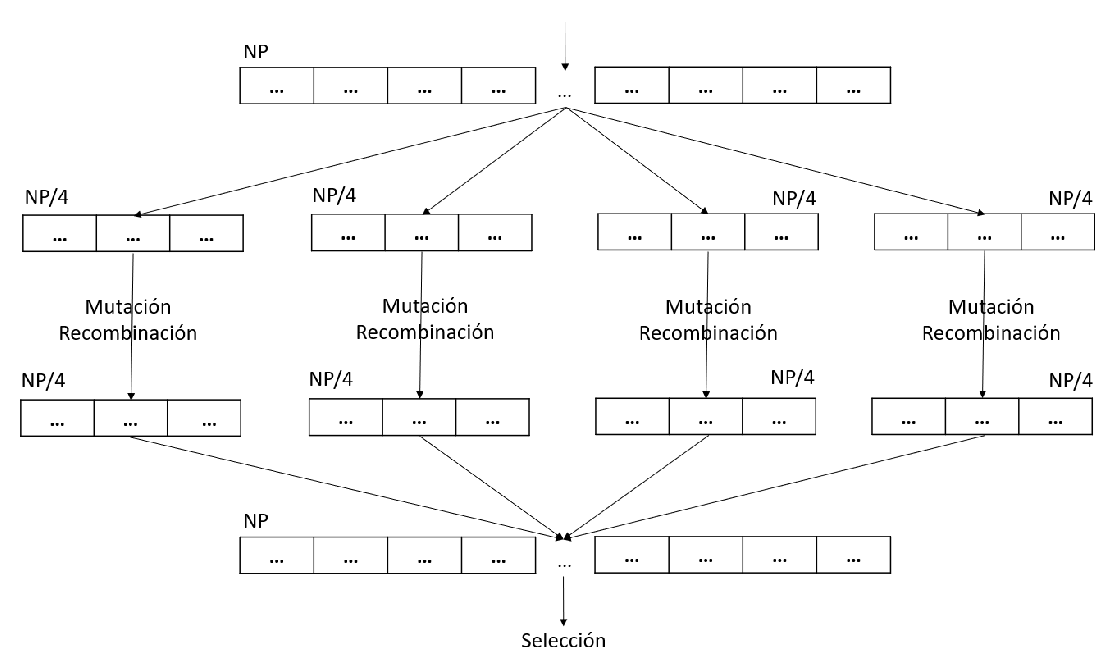
\includegraphics[width=\textwidth]{images/Paralelizacion-DE.eps}
    \caption{Paralelización del algoritmo DE.}
    \label{fig:ParalelizacionDE}
\end{figure}

\begin{figure}[H]
    \centering
    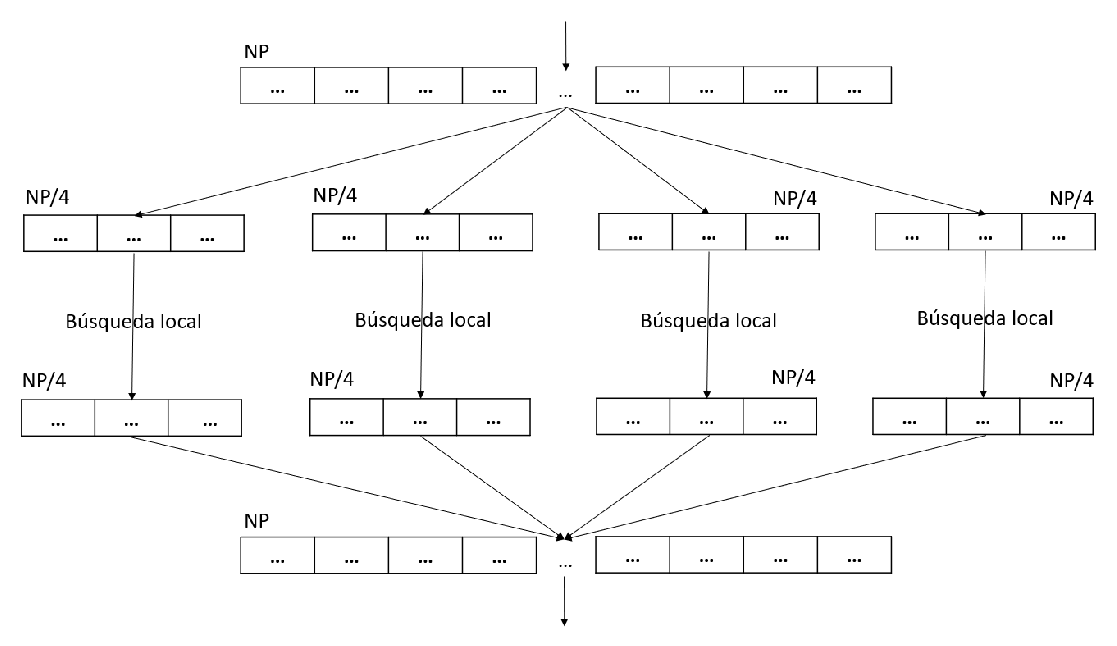
\includegraphics[width=\textwidth]{images/Paralelizacion-LS.eps}
    \caption{Paralelización de la búsqueda local.}
    \label{fig:ParalelizacionLS}
\end{figure}

\section{\textit{HDE} para el \textit{FJSSP}}
El algoritmo \ref{alg:algoritmoDEhibrido} presenta el pseudocódigo del algoritmo de \textit{DE} híbrido para \textit{FJSSP}. Como se puede observar el esquema general es el mismo que el presentado en el capítulo anterior, con la inclusión del proceso de búsqueda local. Además, se agrega como entrada la probabilidad de aplicar búsqueda local ($P_{BL}$), con el fin de permitir al investigador realizar cambios sobre el parámetro.

\begin{algorithm} [H]
    \caption{Pseudocódigo de la Evolución Diferencial (DE)} \label{alg:algoritmoDEhibrido}
    \begin{algorithmic} [1]
    \Require {$F, Cr, N_p, P_{BL}$} 
    \Ensure {$x_{best}$} 
        \State inicializar($P$,$N_p$) 
        \State $g \leftarrow 0$
        \While {no se alcance la condición de fin}
            \For {cada vector $x_{i}^g$ de $P^g$}
                \State $v_{i}^g \leftarrow $ mutación($x_{i}^g, P^g, F$) 
                \State $u_{i}^g \leftarrow $ recombinación($x_{i}^g, v_{i}^g, Cr$)
                \State $x_{i}^{g+1} \leftarrow $ selección($x_{i}^g, u_{i}^g$)
                \State agregar($P^{g+1}, x_{i}^{g+1}$) 
            \EndFor
            \State búsqueda-local($P^g$, $P_{BL}$)
            \State $g \leftarrow g+1$ 
        \EndWhile
        \State$x_{best} \leftarrow $mejor-solución($P^{g}$)

    \end{algorithmic}
\end{algorithm}
    \chapter{Estudios experimentales}
\section{Introducción}
Para validar el algoritmo presentado en esta tesis, se adoptó un conjunto de instancias de prueba del FJSSP, otorgando grandes ventajas a la hora de comparar los resultados obtenidos frente a otros algoritmos. A fin de permitir una comparación cuantitativa de resultados, en este trabajo se utilizaron tablas comparativas que exponen los valores óptimos, los mejores obtenidos y las medias de los mismos, junto con el desvío estándar. Además se utilizó el error relativo, que es el cociente entre el error absoluto de una medida y el valor real de ésta, mostrados en forma de gráficos de caja (\textit{boxplot} en inglés), los cuales son una forma de presentación estadística destinada, fundamentalmente, a resaltar aspectos de la distribución de las observaciones en una o más series de datos cuantitativos. El gráfico de caja es una buena alternativa a la presentación tradicional de datos medidos con escala cuantitativa, pues permite cotejar varias series de datos medidas con la misma escala y ubicadas en posiciones parecidas de ésta, siendo, en tal sentido, más claro y de mayor información que otros tipos de gráficos.


Dado que el objetivo del paralelismo es la reducción del tiempo real, se utiliza la aceleración como medida de comparación del algoritmo \textit{DE} frente a su versión paralela. El tiempo debe incluir cualquier actividad que se realice en el proceso, por lo que la opción más prudente para medir el rendimiento de un código paralelo es considerar el tiempo entre el inicio y fin de todo el algoritmo para resolver el problema en cuestión. Para una comparación justa, la misma idea debe ser tomada en consideración en el caso secuencial.


En este capítulo se describe el diseño experimental llevado a cabo para este trabajo. Además se presentan los resultados experimentales obtenidos variando el factor de escalado ($F$) y la probabilidad de recombinación ($Cr$), agregando el procedimiento de búsqueda local y la mejora en tiempo del algoritmo gracias al paralelismo. Por último, se lleva a cabo una comparación de los resultados del algoritmo \textit{HDE} frente a otros algoritmos competitivos presentes en la literatura.

\section{Diseño experimental}


En esta sección, se describe el diseño experimental utilizado en este trabajo. Se selecciona una amplia gama de instancias del FJSSP utilizadas en la literatura teniendo en cuenta su complejidad, que viene dada por el número de trabajos y máquinas, y la amplia variación de flexibilidad en la cantidad de máquinas disponibles por operación. En este sentido, fue considerado el conjunto de datos propuestos por Brandimarte \cite{Brandimarte} presentado en la tabla \ref{tab:InstanciasBrandirmarte}, ya que el número de trabajos varía de 10 a 20, el número de máquinas pertenece al rango [4,15] y el número de operaciones para cada trabajo puede tomar valores desde 5 a 15, en consecuencia, el número total de operaciones va desde 55 a 255. Teniendo en cuenta la flexibilidad esta oscila entre 1.43 y 4.10 \cite{MinettiSalto}.


% Table generated by Excel2LaTeX from sheet 'Hoja 1'
\begin{table}[!tb]
    \scriptsize
  \centering
  \caption{Instancias propuestas por Brandimarte}
    \begin{tabular}{|c|c|c|c|c|}
    \hline
    \textbf{Instancia} & \textbf{Cantidad de trabajos} & \textbf{Cantidad de operaciones} & \textbf{Cantidad de máquinas} & \textbf{Óptimo} \bigstrut\\
    \hline
    Mk01 & 10  & 55  & 6   & 40 \\
    Mk02 & 10  & 58  & 6   & 26 \\
    Mk03 & 15  & 150 & 8   & 204 \\
    Mk04 & 15  & 90  & 8   & 60 \\
    Mk05 & 15  & 106 & 4   & 172 \\
    Mk06 & 10  & 150 & 15  & 58 \\
    Mk07 & 20  & 100 & 5   & 139 \\
    Mk08 & 20  & 255 & 10  & 523 \\
    Mk09 & 20  & 240 & 10  & 307 \\
    Mk10 & 20  & 240 & 15  & 197 \\
    \hline
    \end{tabular}%
  \label{tab:InstanciasBrandirmarte}%
\end{table}%

Con respecto a la metodología seguida para analizar los resultados, primero, estudiamos el comportamiento de estos algoritmos con diferentes valores de $ Cr$ y $F$, considerando los mejores $ C_ {max} $ encontrados y el error relativo de $ C_ {max} $ contra el óptimo conocido en cada instancia. Estos análisis nos permiten determinar los mejores valores para los parámetros de control. En segundo lugar, determinamos el impacto de incorporar un procedimiento de búsqueda local a diferentes probabilidades $ P_ {BL} $. Para este propósito, tomamos en cuenta los mejores $ C_ {max} $ encontrados, la tasa de aciertos (es decir, la cantidad de veces que un algoritmo encuentra la mejor solución) y el error relativo de $ C_ {max} $ contra el óptimo conocido en cada instancia. Finalmente, estudiamos el comportamiento del algoritmo de \textit{DE} híbrido incluyendo el paralelismo con respecto al tiempo de ejecución en cada enfoque.


Los algoritmos considerados fueron programados en C++, por lo que su tiempo de ejecución es directamente comparable. Todos los algoritmos se compilaron en la misma computadora con los mismos indicadores de compilación y se ejecutaron en hardware homogéneo. La experimentación se llevó a cabo en un clúster conformado por cuatro máquinas con INTEL I7 3770K, 8 GB de RAM y el Slackware Linux con la versión 2.6.27 del núcleo. Para implementar la versión paralela de DE, se utiliza una interfaz de programación de aplicaciones (API) para computadoras paralelas de memoria compartida como es OpenMP \cite{openMP}.


\begin{table}[b]
    \scriptsize
\centering
\caption{Valores de los parámetros}
    \begin{tabular}{|c|c|}
    \hline
    \multicolumn{1}{|c|}{\textbf{Parámetro}} & \multicolumn{1}{c|}{\textbf{Valor}} \\ 
    \hline
    $N_P$                              & 50                          \\
    $F$                               & 0.1, 0.5, y 0.9           \\
    $Cr$                              & 0.1, 0.5, y 0.9                 \\
    $P_{BL}$                          & 0.1, 0.5, y 0.7          \\
    \hline
    \end{tabular}
\label{tab:DEparameteres}%
\end{table}


Para este estudio, la configuración paramétrica del DE es la que se muestra en la tabla \ref{tab:DEparameteres}. El tamaño de la población, $ N_P $, fue adoptado de trabajos anteriores y se establece en 50. Con respecto a la probabilidad de $Cr$ y el factor $F$, se consideraron tres valores diferentes para cada uno de ellos 0.1, 0.5 y 0.9.
Utilizar un valor de $Cr$ alto implica que el vector prueba hereda muchos componentes del vector donador. En caso contrario, si es muy bajo, el vector prueba hereda muchos componentes del vector objetivo. Un valor intermedio como el de 0.5, produciría una situación intermedia e incrementaría la diversidad poblacional. Los valores extremos harían que la diversidad poblacional no fuese incrementada.
El factor de escalado $F$ controla la longitud del salto generado en la explotación del espacio de búsqueda. Un valor bajo lleva al algoritmo a intensificar la explotación de soluciones en algunas regiones del espacio de búsqueda, mientras que un valor alto implica una mayor diversificacion de las soluciones, explorando en mayor medida todo el espacio de búsqueda. Un valor intermedio hace un balance entre diversificación e intensificación.
Para el parámetro restante, $ P_{BL} $, también se analizaron tres valores 0.1, 0.5 y 0.7 (valores con baja, media y alta probabilidad), para estudiar cómo la frecuencia de aplicación de la búsqueda local impacta en los resultados arrojados por el \textit{DE}.


Para hacer una comparación justa entre estos algoritmos, deben hacer el mismo esfuerzo computacional en cada ejecución. Puede lograrse si se ejecuta durante el mismo tiempo cada instancia del problema. De esta manera, el tiempo total ejecutado para una instancia se calcula teniendo en cuenta su tamaño. En la Ecuación \ref{eqtime2} se explica cómo se calcula el tiempo total de ejecución, donde $\sharp O $ es el cantidad de operaciones para una instancia determinada.

\begin{equation}\label{eqtime2}
TiempoEjecucion = \sharp O \times (\frac{\sharp O}{2})\times 30 
\end{equation}

Debido a la naturaleza estocástica de los algoritmos, fueron realizadas 30 ejecuciones independientes de cada prueba con el fin de recopilar datos experimentales significativos y aplicar métricas de confianza estadística para validar las conclusiones.


\section{Resultados experimentales}

En esta sección, analizamos la calidad de los resultados considerando los valores de $ C_ {max} $ obtenidos para las distintas mejoras planteadas al algoritmo DE descrito en el capítulo anterior para resolver las instancias de FJSSP.
En primer lugar se estudiará la influencia de los parámetros $Cr$ y $F$, luego la incorporación del proceso de búsqueda local a través del parámetro $P_{BL}$, después el impacto en los tiempos al incorporar un paralelismo a nivel de iteración y por último se hace una comparación de los valores de $ C_ {max} $ obtenidos por el algoritmo con los alcanzados por varios algoritmos competitivos presentes en la literatura. 


\subsection{Resultados variando los parámetros $F$ y $Cr$ }

El primer análisis se centra en el efecto de usar diferentes valores de $F$ y $Cr$ en el rendimiento de \textit{DE}, de valores bajos a altos (0.1, 0.5 y 0.9). Para este fin, se analizó la calidad de los resultados teniendo en cuenta los valores de $C_{max}$ obtenidos para el \textit{DE} básico al resolver las instancias FJSSP, es decir, se estudió cómo impacta en el rendimiento de \textit{DE} el utilizar las distintas combinaciones de valores de parámetros.


La tabla \ref{tab:resultadosDE} muestra los mejores valores de $C_{max}$ obtenidos para el \textit{DE} utilizando las combinaciones posibles de valores de $F$ y $Cr$ para cada instancia. La columna 2 presenta el mejor valor conocido de $C_{max}$ (óptimo) para cada instancia. La última fila de esta tabla muestra la relación entre el número de instancias resueltas de forma óptima con respecto al número total de instancias. En la tabla \ref{tab:resultadosDEmedias} se encuentran los valores medios de $C_{max}$ junto con la desviación estándar media para los distintos valores de $F$ y $Cr$. 


\begin{table}[t]
    \scriptsize
  \centering
  \caption{Mejores valores de $C_{max}$ encontrados por el \textit{DE} con diferentes valores de $F$ y $Cr$ para todas las instancias del FJSSP}
    \begin{tabular}{|rrccccccccc|}
    \hline
    \multicolumn{1}{|c|}{\multirow{}} & \multicolumn{1}{c|}{\multirow{}} & \multicolumn{9}{c|}{\textbf{Mejor valor de C_{max}}} \bigstrut\\
\cline{3-11}    \multicolumn{1}{|c|}{{\textbf{Instancia}}} & \multicolumn{1}{c|}{{\textbf{Opt.}}} & \multicolumn{1}{c|}{\textbf{F=0.1}} & \multicolumn{1}{c|}{\textbf{F=0.1}} & \multicolumn{1}{c|}{\textbf{F=0.1}} & \multicolumn{1}{c|}{\textbf{F=0.5}} & \multicolumn{1}{c|}{\textbf{F=0.5}} & \multicolumn{1}{c|}{\textbf{F=0.5}} & \multicolumn{1}{c|}{\textbf{F=0.9}} & \multicolumn{1}{c|}{\textbf{F=0.9}} & \multicolumn{1}{c|}{\textbf{F=0.9}} \\
    \multicolumn{1}{|c|}{} & \multicolumn{1}{c|}{} & \multicolumn{1}{c|}{\textbf{Cr=0.1}} & \multicolumn{1}{c|}{\textbf{Cr=0.5}} & \multicolumn{1}{c|}{\textbf{Cr=0.9}} & \multicolumn{1}{c|}{\textbf{Cr=0.1}} & \multicolumn{1}{c|}{\textbf{Cr=0.5}} & \multicolumn{1}{c|}{\textbf{Cr=0.9}} & \multicolumn{1}{c|}{\textbf{Cr=0.1}} & \multicolumn{1}{c|}{\textbf{Cr=0.5}} & \multicolumn{1}{c|}{\textbf{Cr=0.9}} \\
    \hline
    \multicolumn{1}{|c|}{Mk01} & \multicolumn{1}{c|}{40} & \multicolumn{1}{c|}{\textbf{40}} & \multicolumn{1}{c|}{\textbf{40}} & \multicolumn{1}{c|}{\textbf{40}} & \multicolumn{1}{c|}{\textbf{40}} & \multicolumn{1}{c|}{\textbf{40}} & \multicolumn{1}{c|}{\textbf{40}} & \multicolumn{1}{c|}{\textbf{40}} & \multicolumn{1}{c|}{\textbf{40}} & \textbf{40} \bigstrut\\
    %\hline
    \multicolumn{1}{|c|}{Mk02} & \multicolumn{1}{c|}{26} & \multicolumn{1}{c|}{\textbf{26}} & \multicolumn{1}{c|}{27} & \multicolumn{1}{c|}{27} & \multicolumn{1}{c|}{\textbf{26}} & \multicolumn{1}{c|}{27} & \multicolumn{1}{c|}{\textbf{26}} & \multicolumn{1}{c|}{27} & \multicolumn{1}{c|}{27} & 27 \bigstrut\\
    %\hline
    \multicolumn{1}{|c|}{Mk03} & \multicolumn{1}{c|}{204} & \multicolumn{1}{c|}{\textbf{204}} & \multicolumn{1}{c|}{\textbf{204}} & \multicolumn{1}{c|}{\textbf{204}} & \multicolumn{1}{c|}{\textbf{204}} & \multicolumn{1}{c|}{\textbf{204}} & \multicolumn{1}{c|}{\textbf{204}} & \multicolumn{1}{c|}{\textbf{204}} & \multicolumn{1}{c|}{\textbf{204}} & \textbf{204} \bigstrut\\
    %\hline
    \multicolumn{1}{|c|}{Mk04} & \multicolumn{1}{c|}{60} & \multicolumn{1}{c|}{\textbf{60}} & \multicolumn{1}{c|}{\textbf{60}} & \multicolumn{1}{c|}{65} & \multicolumn{1}{c|}{61} & \multicolumn{1}{c|}{\textbf{60}} & \multicolumn{1}{c|}{\textbf{60}} & \multicolumn{1}{c|}{62} & \multicolumn{1}{c|}{63} & 62 \bigstrut\\
    %\hline
    \multicolumn{1}{|c|}{Mk05} & \multicolumn{1}{c|}{172} & \multicolumn{1}{c|}{175} & \multicolumn{1}{c|}{173} & \multicolumn{1}{c|}{173} & \multicolumn{1}{c|}{175} & \multicolumn{1}{c|}{179} & \multicolumn{1}{c|}{173} & \multicolumn{1}{c|}{175} & \multicolumn{1}{c|}{179} & 173 \bigstrut\\
    %\hline
    \multicolumn{1}{|c|}{Mk06} & \multicolumn{1}{c|}{58} & \multicolumn{1}{c|}{65} & \multicolumn{1}{c|}{59} & \multicolumn{1}{c|}{63} & \multicolumn{1}{c|}{66} & \multicolumn{1}{c|}{69} & \multicolumn{1}{c|}{59} & \multicolumn{1}{c|}{67} & \multicolumn{1}{c|}{70} & 61 \bigstrut\\
    %\hline
    \multicolumn{1}{|c|}{Mk07} & \multicolumn{1}{c|}{139} & \multicolumn{1}{c|}{143} & \multicolumn{1}{c|}{140} & \multicolumn{1}{c|}{142} & \multicolumn{1}{c|}{143} & \multicolumn{1}{c|}{148} & \multicolumn{1}{c|}{140} & \multicolumn{1}{c|}{144} & \multicolumn{1}{c|}{146} & 140 \bigstrut\\
    %\hline
    \multicolumn{1}{|c|}{Mk08} & \multicolumn{1}{c|}{523} & \multicolumn{1}{c|}{\textbf{523}} & \multicolumn{1}{c|}{\textbf{523}} & \multicolumn{1}{c|}{\textbf{523}} & \multicolumn{1}{c|}{\textbf{523}} & \multicolumn{1}{c|}{\textbf{523}} & \multicolumn{1}{c|}{\textbf{523}} & \multicolumn{1}{c|}{\textbf{523}} & \multicolumn{1}{c|}{\textbf{523}} & \textbf{523} \bigstrut\\
    %\hline
    \multicolumn{1}{|c|}{Mk09} & \multicolumn{1}{c|}{307} & \multicolumn{1}{c|}{318} & \multicolumn{1}{c|}{\textbf{307}} & \multicolumn{1}{c|}{310} & \multicolumn{1}{c|}{321} & \multicolumn{1}{c|}{333} & \multicolumn{1}{c|}{\textbf{307}} & \multicolumn{1}{c|}{321} & \multicolumn{1}{c|}{338} & \textbf{307} \bigstrut\\
    %\hline
    \multicolumn{1}{|c|}{Mk10} & \multicolumn{1}{c|}{197} & \multicolumn{1}{c|}{237} & \multicolumn{1}{c|}{210} & \multicolumn{1}{c|}{221} & \multicolumn{1}{c|}{238} & \multicolumn{1}{c|}{245} & \multicolumn{1}{c|}{206} & \multicolumn{1}{c|}{240} & \multicolumn{1}{c|}{246} & 215 \bigstrut\\
    \hline
        &     & 5/10 & 5/10 & 3/10 & 4/10 & 4/10 & 6/10 & 3/10 & 3/10 & 4/10 \bigstrut\\
    \hline
    \end{tabular}%
\label{tab:resultadosDE}
\end{table}%

% Table generated by Excel2LaTeX from sheet 'DE media y sd'

\begin{table}[!tb]
   \scriptsize
  \centering
  \caption{Valores medios de $C_{max}$ encontrados por el \textit{DE} con diferentes valores de $F$ y $Cr$ para todas las instancias del FJSSP}
    \begin{adjustbox}{max width=\textwidth}
    \begin{tabular}{|c|c|c|c|c|c|c|c|c|c|}
    \hline
    \multirow{} & \multicolumn{9}{c|}{\textbf{Valor medio de Cmax y desvío estándar medio }} \\
\cline{2-10}   \textbf{Instancia}     & \multicolumn{1}{c|}{\textbf{F=0,1}} & \multicolumn{1}{c|}{\textbf{F=0.1}} & \multicolumn{1}{c|}{\textbf{F=0.1}} & \multicolumn{1}{c|}{\textbf{F=0.5}} & \multicolumn{1}{c|}{\textbf{F=0.5}} & \multicolumn{1}{c|}{\textbf{F=0.5}} & \multicolumn{1}{c|}{\textbf{F=0.9}} & \multicolumn{1}{c|}{\textbf{F=0.9}} & \multicolumn{1}{c|}{\textbf{F=0.9}} \\
        & \multicolumn{1}{c|}{\textbf{Cr=0.1}} & \multicolumn{1}{c|}{\textbf{Cr=0.5}} & \multicolumn{1}{c|}{\textbf{Cr=0.9}} & \multicolumn{1}{c|}{\textbf{Cr=0.1}} & \multicolumn{1}{c|}{\textbf{Cr=0.5}} & \multicolumn{1}{c|}{\textbf{Cr=0.9}} & \multicolumn{1}{c|}{\textbf{Cr=0.1}} & \multicolumn{1}{c|}{\textbf{Cr=0.5}} & \multicolumn{1}{c|}{\textbf{Cr=0.9}} \bigstrut\\
    \hline
    Mk01 & 40 $_{\pm  0.00}$ & 40.26$_{\pm 0.69 }$& 41.8$_{\pm 0.48 }$& 40$_{\pm 0.00 & 4}$0$_{\pm 0.00 & 4}$0.06$_{\pm 0.25 }$& 40$_{\pm 0.00 & 4}$0.03$_{\pm 0.18 }$& 40.53$_{\pm 0.73 }$\bigstrut\\
    %\hline
    Mk02 & 26.57 $_{\pm  0.50}$ & 27$_{\pm 0.00 & 2}$7.8$_{\pm 0.48 }$& 26.96$_{\pm 0.18 }$& 27.33$_{\pm 0.47 }$& 26.96$_{\pm 0.18 }$& 27.03$_{\pm 0.18 }$& 27.23$_{\pm 0.43 }$& 27.33$_{\pm 0.47 }$\bigstrut\\
    %\hline
    Mk03 & 204 $_{\pm  0.00}$ & 204$_{\pm 0.00 & 2}$04$_{\pm 0.00 & 2}$04$_{\pm 0.00 & 2}$04$_{\pm 0.00 & 2}$04$_{\pm 0.00 & 2}$04$_{\pm 0.00 & 2}$04$_{\pm 0.00 & 2}$04$_{\pm 0.00}$\bigstrut\\
    %\hline
    Mk04 & 60 $_{\pm  0.00}$ & 62.03$_{\pm 1.42 }$& 66.93$_{\pm 0.82 }$& 62.16$_{\pm 0.53 }$& 65.76$_{\pm 1.27 }$& 64.56$_{\pm 1.90 }$& 63.76$_{\pm 0.97 }$& 66.23$_{\pm 0.81 }$& 65.33$_{\pm 1.72 }$\bigstrut\\
    %\hline
    Mk05 & 176.33 $_{\pm  0.66}$ & 177.2$_{\pm 1.67 }$& 175.8$_{\pm 1.07 }$& 176.5$_{\pm 0.73 }$& 181.3$_{\pm 0.96 }$& 173.6$_{\pm 0.92 }$& 176.8$_{\pm 0.69 }$& 181.2$_{\pm 1.01 }$& 173.7$_{\pm 0.94 }$\bigstrut\\
    %\hline
    Mk06 & 66.7 $_{\pm 0.75 }$& 64.2$_{\pm 2.52 }$& 66.13$_{\pm 1.04 }$& 67.53$_{\pm 0.62 }$& 70.83$_{\pm 0.69 }$& 61.93$_{\pm 1.36 }$& 67.96$_{\pm 0.55 }$& 71.1$_{\pm 0.54 }$& 63.53$_{\pm 1.19 }$\bigstrut\\
    %\hline
    Mk07 & 144.3 $_{\pm  0.53}$ & 143.8$_{\pm 2.02 }$& 144.5$_{\pm 1.27 }$& 144.5$_{\pm 0.77 }$& 150.1$_{\pm 0.94 }$& 141.8$_{\pm 1.39 }$& 144.8$_{\pm 0.79 }$& 150.1$_{\pm 1.11 }$& 142.1$_{\pm 1.12 }$\bigstrut\\
    %\hline
    Mk08 & 523 $_{\pm  0.00}$ & 523$_{\pm 0.00 & 5}$23$_{\pm 0.00 & 5}$23$_{\pm 0.00 & 5}$23.5$_{\pm 1.04 }$& 523$_{\pm 0.00 & 5}$23$_{\pm 0.00 & 5}$23.6$_{\pm 0.95 }$& 523$_{\pm 0.00}$\bigstrut\\
    %\hline
    Mk09 & 323.6 $_{\pm  2.44}$ & 316.1$_{\pm 7.98 }$& 323.9$_{\pm 6.23 }$& 326.3$_{\pm 2.35 }$& 341.5$_{\pm 2.87 }$& 307.5$_{\pm 1.47 }$& 327.9$_{\pm 2.32 }$& 342.3$_{\pm 2.29 }$& 310.7$_{\pm 3.46 }$\bigstrut\\
    %\hline
    Mk10 & 240.63 $_{\pm  1.54}$ & 239.5$_{\pm 7.10 }$& 226.8$_{\pm 2.83 }$& 242.1$_{\pm 1.85 }$& 251.2$_{\pm 2.12 }$& 212.4$_{\pm 2.99 }$& 242.3$_{\pm 1.32 }$& 251.7$_{\pm 1.86 }$& 219.5$_{\pm 2.66 }$\bigstrut\\
    \hline
    \end{tabular}%
    \end{adjustbox}
\label{tab:resultadosDEmedias}
\end{table}%

Como se puede ver en la Tabla \ref{tab:resultadosDE},  el \textit{DE} encuentra el óptimo en 3 instancias (MK01, MK03 y MK08) independientemente de las combinaciones de valores de $F$ y $Cr$ consideradas. Con un valor alto de $F$ \textit{DE} tiene menos posibilidades de encontrar las mejores soluciones para el FJSSP sin importar el valor de $Cr$ usado, ya que la cantidad de valores óptimos alcanzados para las diferentes instancias es menor frente a otras posibles combinaciones de valores paramétricos (no más de 4 de las 10 instancias). El \textit{DE} con $F = 0.5 $ y $Cr = 0.9 $ encuentra una mayor cantidad de veces valores de $ C_ {max} $ óptimos que el resto de las combinaciones (en 6 de las 10 instancias).


Una métrica importante es el error relativo de los mejores $ C_ {max} $ obtenidos para cada instancia con respecto al óptimo. Esta métrica nos permite normalizar los datos de las diferentes instancias y, de esta manera, enfocar la atención en cómo las diferentes combinaciones de valores de $F$ y $Cr$ afectan al rendimiento de \textit{DE} al resolver el FJSSP. Observando el \textit{boxplot} del error relativo para las distintas combinaciones de parámetros de $F$ y $Cr$ presentado en la Figura \ref{fig:DEboxplot} se puede ver que el algoritmo \textit{DE} con $F = 0.5 $ y $Cr = 0.9 $ presenta la menor mediana del error. La caja de rango intercuartil muestra que la distancia entre el primer cuartil y el tercer cuartil es menor frente a otras posibles combinaciones de valores de parámetros. Los bigotes que se extienden desde la parte superior de la caja son claramente inferiores frente a los de las demás combinaciones. Por último, se puede observar que no existen valores atípicos, lo cual presenta una superioridad con respecto a las posibles elecciones de parámetros. 

\begin{figure}[H]
   \scriptsize
    \centering
    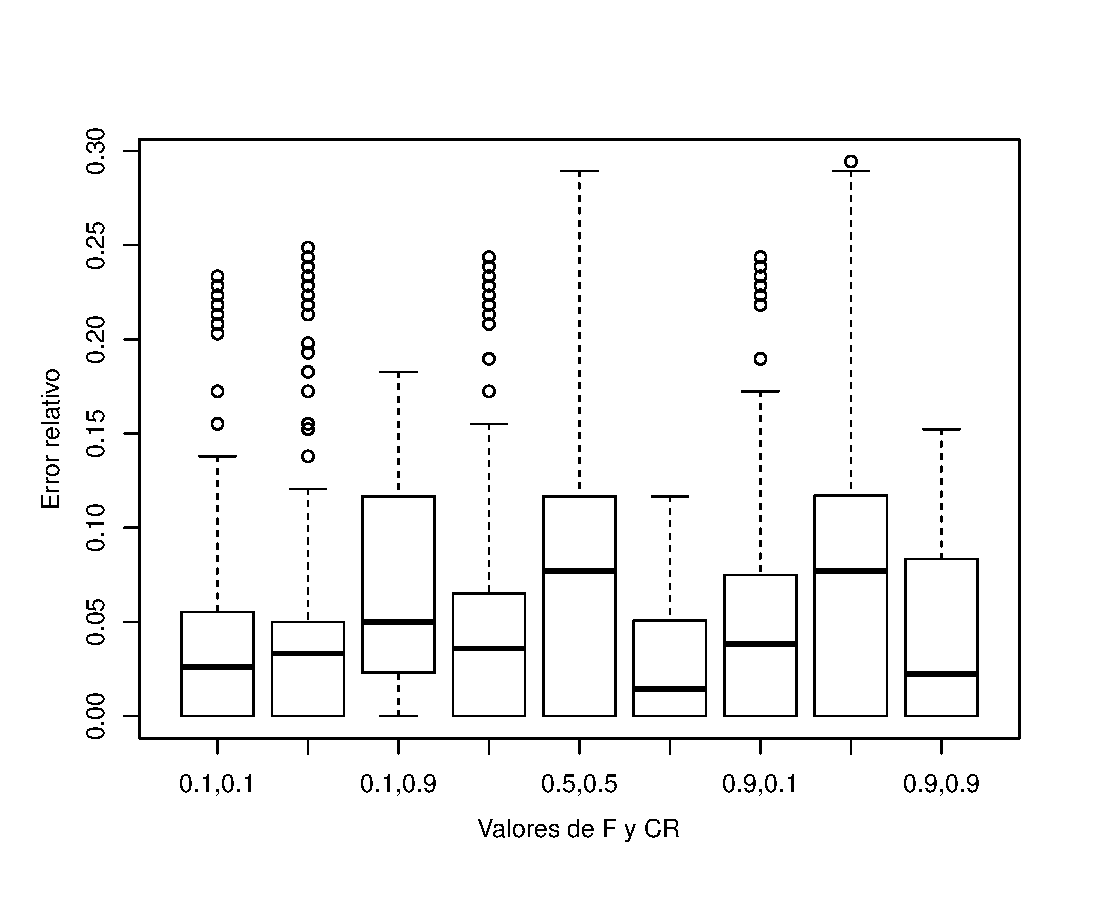
\includegraphics[trim={0 1cm 0 0.8cm},scale=0.6]{images/Boxplot-DE.eps}
    \caption{Boxplot del error relativo del \textit{DE} para distintos valores de $F$ y $Cr$.}
    \label{fig:DEboxplot}
\end{figure}


Finalmente, se estudiará la distribución del número de evaluaciones realizadas por \textit{DE} para encontrar los mejores valores de $ C_ {max} $ para las diferentes combinaciones de $F$ y $Cr$. Con este fin, la Figura \ref{fig:DE10boxplot} ilustra los resultados utilizando diez \textit{boxplots} (uno por cada instancia). En general, se observa que el algoritmo \textit{DE} con menor cantidad de evaluaciones es aquel con $F\in \{0.1,0.5\}$ y $Cr=0.9$, pero la combinación $F = 0.5 $ y $Cr = 0.9 $ supera a las demás desde el punto de vista de la calidad de resultados (ver Tabla \ref{tab:resultadosDE}). En consecuencia, serán considerados los valores de $F = 0.5 $ y $Cr = 0.9 $ en la experimentación restante.

\begin{figure}[H]
   \scriptsize
    \centering
    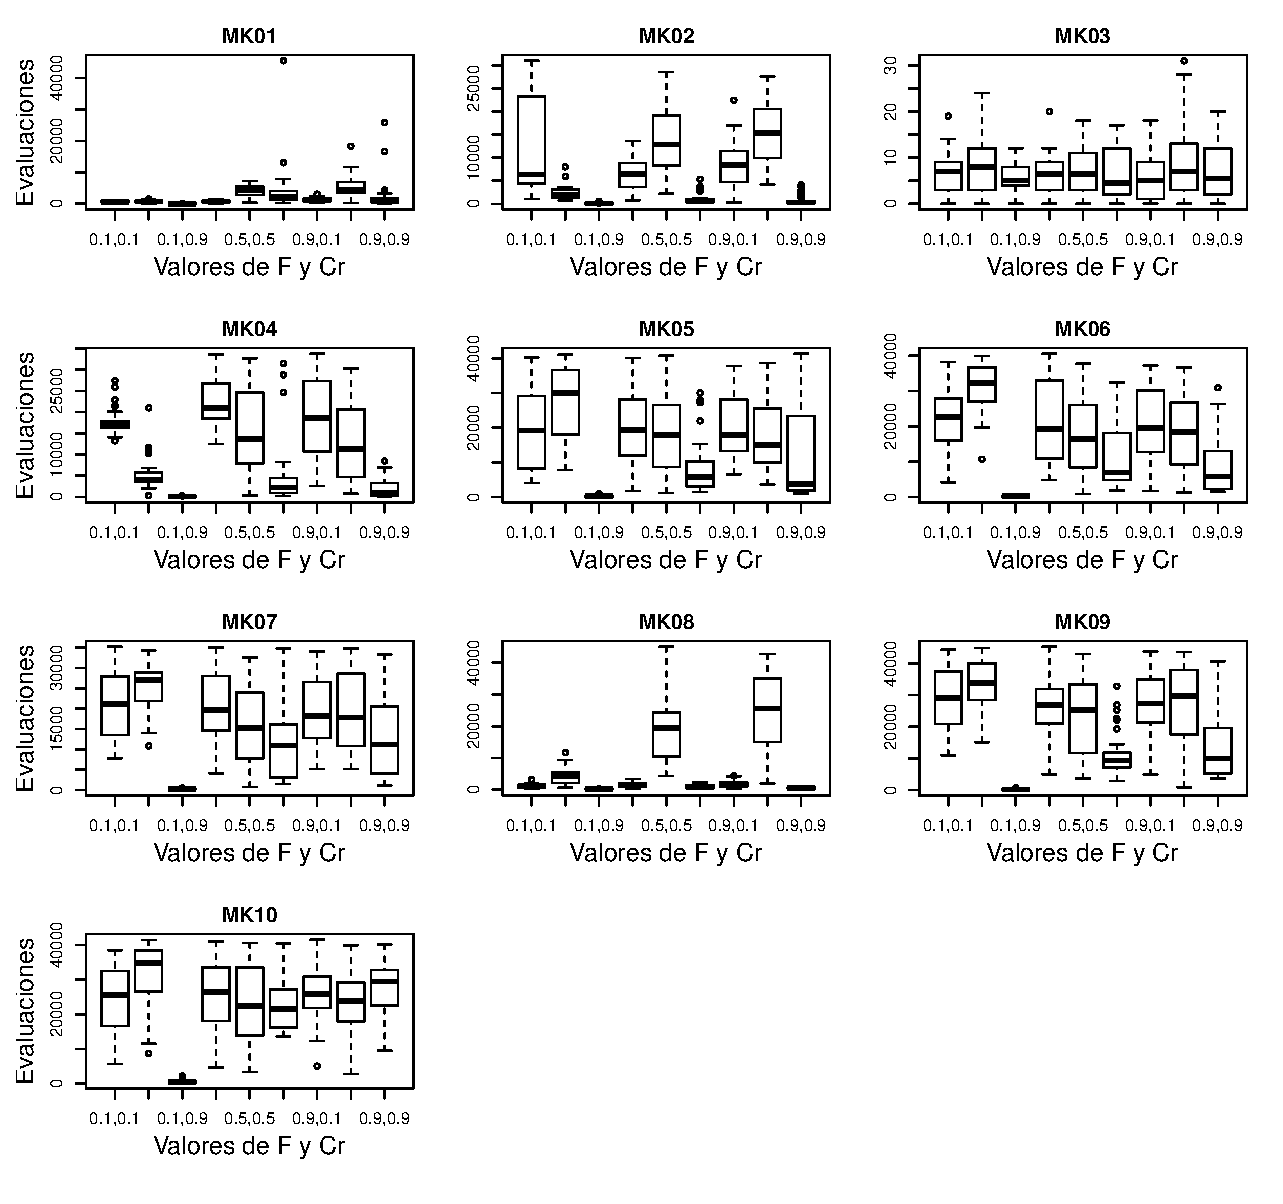
\includegraphics[trim={0 0.6cm 0 0cm},scale=0.7]{images/DE-10boxplot.eps}
    \caption{Boxplot del error relativo del \textit{DE} para distintos valores de $F$ y $Cr$.}
    \label{fig:DE10boxplot}
\end{figure}


\subsection{Resultados de \textit{DE} con búsqueda local}
En esta sub-sección se analiza en detalle lo que sucede al introducir un procedimiento de búsqueda local en el algoritmo \textit{DE} para resolver las instancias de FJSSP. El algoritmo resultante es llamado \textit{HDE}. Para esos estudios, fueron considerados tres valores diferentes de $P_{BL}$: 0.1, 0.5 y 0.7 (de valores altos a bajos), es decir, se estudió cómo la frecuencia de la aplicación del procedimiento de búsqueda local impacta en el rendimiento de \textit{HDE}.


La tabla \ref{tab:tableDELS} muestra los mejores y la media de los valores de $C_{max}$ obtenidos para el algoritmo \textit{HDE} con los diferentes valores de $P_{BL}$. El algoritmo \textit{HDE} obtiene un número mayor de $C_{max}$ óptimos con $P_{BL} = 0.5$ y con $P_{BL} = 0.7$. Pero el algoritmo \textit{HDE} que aplica el procedimiento de búsqueda local con la frecuencia más alta ($P_{BL} = 0.7$) presenta valores de $C_{max}$ medios más bajo para todas las instancias. Esto indica que el algoritmo encuentra el valor óptimo o casi óptimo en la mayoría de las ejecuciones, lo cual queda claramente plasmado en el \textit{boxplot} del error relativo de las distintas instancias contra los óptimos para los distintos valores de $P_{BL}$ presentado en la figura ~\ref{fig:DELSboxplot}, donde se observa que la mediana del error es menor con la frecuencia de búsqueda local más alta.


% Table generated by Excel2LaTeX from sheet 'Hoja1'
\begin{table}[!tb]
  \centering
     \scriptsize
    \caption{Valores de $C_{max}$ encontrados por el \textit{HDE} con diferentes valores de $P_{BL}$ para todas las instancias de FJSSP.}
    \begin{tabular}{|rrcccrrc|}
    \hline
    \multicolumn{1}{|c|}{\multirow{}{\textbf{Instancia}}} & \multicolumn{1}{c|}{\multirow{}{\textbf{Optimos}}} & \multicolumn{3}{c|}{\textbf{Mejor valor de Cmax}} & \multicolumn{3}{c|}{\textbf{Valor medio de Cmax y desvío estándar medio }} \bigstrut\\
\cline{3-8}    \multicolumn{1}{|c|}{} & \multicolumn{1}{c|}{} & \multicolumn{1}{c|}{\textbf{$P_{BL}=0.1$}} & \multicolumn{1}{c|}{\textbf{$P_{BL}=0.5$}} & \multicolumn{1}{c|}{\textbf{$P_{BL}=0.7$}} & \multicolumn{1}{c|}{\textbf{$P_{BL}=0.1$}} & \multicolumn{1}{c|}{\textbf{$P_{BL}=0.5$}} & \multicolumn{1}{c|}{\textbf{$P_{BL}=0.7$}} \bigstrut\\
    \hline
    \multicolumn{1}{|c|}{Mk01} & \multicolumn{1}{c|}{40} & \multicolumn{1}{c|}{\textbf{40}} & \multicolumn{1}{c|}{\textbf{40}} & \multicolumn{1}{c|}{\textbf{40}} & \multicolumn{1}{c|}{40$_{\pm 0.00}$} & \multicolumn{1}{c|}{40$_{\pm 0.00}$} & 40$_{\pm 0.00}$ \bigstrut\\
    %\hline
    \multicolumn{1}{|c|}{Mk02} & \multicolumn{1}{c|}{26} & \multicolumn{1}{c|}{27} & \multicolumn{1}{c|}{\textbf{26}} & \multicolumn{1}{c|}{\textbf{26}} & \multicolumn{1}{c|}{27.03$_{\pm 0.18}$} & \multicolumn{1}{c|}{26.96$_{\pm 0.18}$} & 26.76$_{\pm 0.43}$ \bigstrut\\
    %\hline
    \multicolumn{1}{|c|}{Mk03} & \multicolumn{1}{c|}{204} & \multicolumn{1}{c|}{\textbf{204}} & \multicolumn{1}{c|}{\textbf{204}} & \multicolumn{1}{c|}{\textbf{204}} & \multicolumn{1}{c|}{204$_{\pm 0.00}$} & \multicolumn{1}{c|}{204$_{\pm 0.00}$} & 204$_{\pm 0.00}$ \bigstrut\\
    %\hline
    \multicolumn{1}{|c|}{Mk04} & \multicolumn{1}{c|}{60} & \multicolumn{1}{c|}{\textbf{60}} & \multicolumn{1}{c|}{\textbf{60}} & \multicolumn{1}{c|}{\textbf{60}} & \multicolumn{1}{c|}{62$_{\pm 1.31}$} & \multicolumn{1}{c|}{61.3$_{\pm 0.70}$} & 61.03$_{\pm 0.66}$ \bigstrut\\
    %\hline
    \multicolumn{1}{|c|}{Mk05} & \multicolumn{1}{c|}{172} & \multicolumn{1}{c|}{173} & \multicolumn{1}{c|}{173} & \multicolumn{1}{c|}{173} & \multicolumn{1}{c|}{174.3$_{\pm 0.75}$} & \multicolumn{1}{c|}{173$_{\pm 0.00}$ }& 173$_{\pm 0.00}$ \bigstrut\\
    %\hline
    \multicolumn{1}{|c|}{Mk06} & \multicolumn{1}{c|}{58} & \multicolumn{1}{c|}{63} & \multicolumn{1}{c|}{62} & \multicolumn{1}{c|}{61} & \multicolumn{1}{c|}{64.4$_{\pm 0.56}$} & \multicolumn{1}{c|}{62.83$_{\pm 0.53}$} & 62.43$_{\pm 0.62}$ \bigstrut\\
    %\hline
    \multicolumn{1}{|c|}{Mk07} & \multicolumn{1}{c|}{139} & \multicolumn{1}{c|}{142} & \multicolumn{1}{c|}{140} & \multicolumn{1}{c|}{140} & \multicolumn{1}{c|}{143.2$_{\pm 0.69}$} & \multicolumn{1}{c|}{142.0$_{\pm 0.90}$} & 141.8$_{\pm 0.92}$ \bigstrut\\
    %\hline
    \multicolumn{1}{|c|}{Mk08} & \multicolumn{1}{c|}{523} & \multicolumn{1}{c|}{\textbf{523}} & \multicolumn{1}{c|}{\textbf{523}} & \multicolumn{1}{c|}{\textbf{523}} & \multicolumn{1}{c|}{523$_{\pm 0.00}$} & \multicolumn{1}{c|}{523$_{\pm 0.00}$} & 523$_{\pm 0.00}$ \bigstrut\\
    %\hline
    \multicolumn{1}{|c|}{Mk09} & \multicolumn{1}{c|}{307} & \multicolumn{1}{c|}{309} & \multicolumn{1}{c|}{\textbf{307}} & \multicolumn{1}{c|}{\textbf{307}} & \multicolumn{1}{c|}{313.1$_{\pm 2.20}$} & \multicolumn{1}{c|}{310.0$_{\pm 1.33}$} & 309.0$_{\pm 1.72}$ \bigstrut\\
    %\hline
    \multicolumn{1}{|c|}{Mk10} & \multicolumn{1}{c|}{197} & \multicolumn{1}{c|}{226} & \multicolumn{1}{c|}{225} & \multicolumn{1}{c|}{224} & \multicolumn{1}{c|}{231.1$_{\pm 2.41}$} & \multicolumn{1}{c|}{228.0$_{\pm 1.36}$} & 227.2$_{\pm 1.38}$ \bigstrut\\
    \hline
          &       & 4/10  & 6/10  & 6/10  &       &       &  \bigstrut\\
    \hline
    \end{tabular}%
    \label{tab:tableDELS}
\end{table}%


Para determinar que el \textit{HDE} presenta una mejora en los valores de $C_{max}$ obtenidos por el \textit{DE}, se realiza una comparación de los valores de los errores relativos mostrados en la Figura \ref{fig:DEboxplot} y los encontrados en la Figura \ref{fig:DELSboxplot}. Se observa que el algoritmo \textit{HDE} con $P_{BL} = 0.7$ presenta menor error relativo frente a los otros presentados en \textit{DE}, lo que indica la ventaja de incorporar la búsqueda local dentro del marco de \textit{DE}.


\begin{figure}[H]
    \centering
    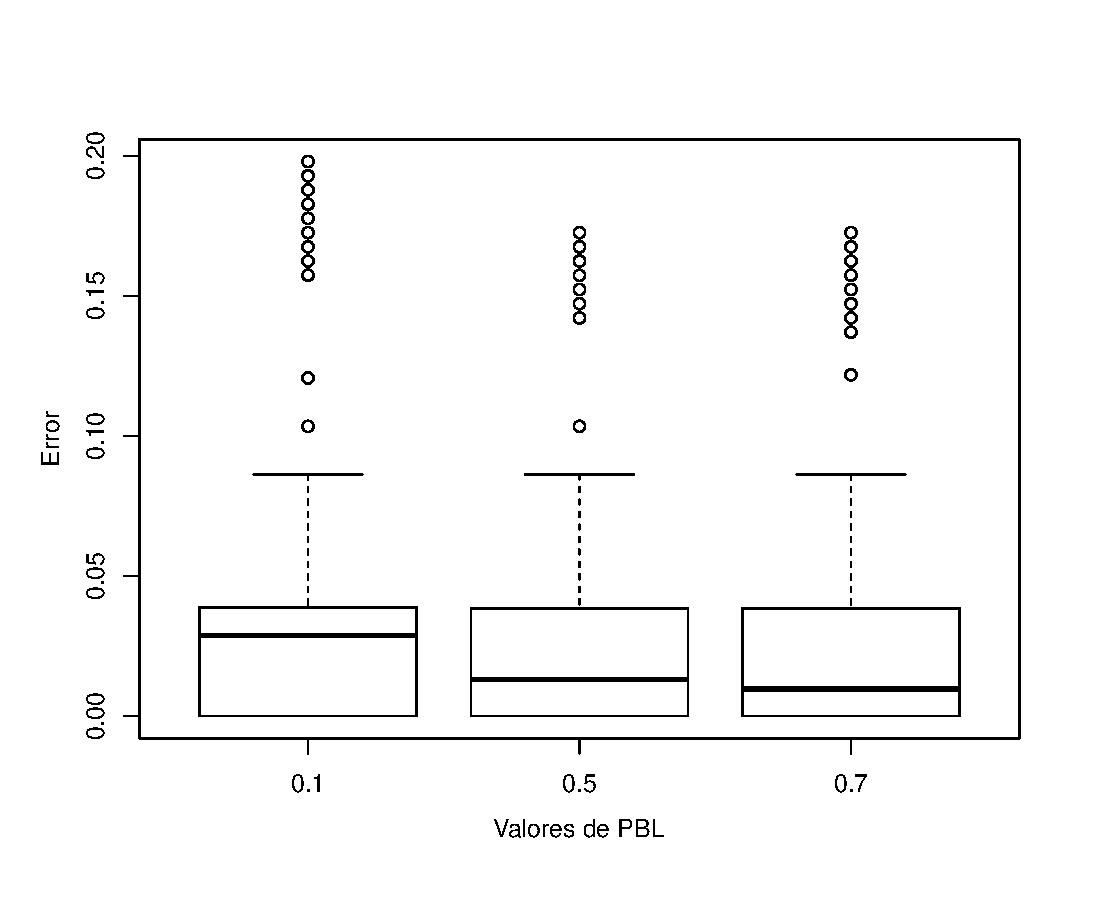
\includegraphics[trim={0 1cm 0 0.8cm},scale=0.6]{images/Boxplot-DELS.eps}
    \caption{Boxplot del error relativo del \textit{HDE} para distintos valores de $P_{BL}$.}
    \label{fig:DELSboxplot}
\end{figure}


\subsection{Resultados de \textit{HDE} y su paralelismo}

En esta subsección se compara el \textit{HDE} contra su versión paralela. La medida más importante de un algoritmo paralelo es el \textit{speedup}. El \textit{speedup} se define como la relación entre el tiempo de ejecución secuencial (tiempo de ejecución de \textit{HDE}, en este caso) y el tiempo de ejecución paralelo. Para este análisis, fue considerado el \textit{speedup} débil \cite{albaMeta2005}. Por esa razón y siguiendo las mejores prácticas de Luque y Alba \cite{LuqueAlba}, el criterio de detención se basa en la calidad de la solución final lograda por los algoritmos, que se establece en los mejores $C_{max}$ conocidos para cada instancia de FJSSP (consulte la columna óptimo de la tabla \ref{tab:InstanciasBrandirmarte}). En consecuencia, los valores de \textit{speedup} solo se informan para las instancias para las cuales el algoritmo \textit{HDE} obtiene el valor óptimo.

 
Una vez establecidos los tiempos de ejecución del algoritmo \textit{HDE} y el algoritmo \textit{HDE} paralelo, se calculan los valores de \textit{speedup}. La Figura \ref{fig:speedup} muestra que el uso de la paralelización vale la pena, ya que permite acelerar el tiempo de ejecución con respecto al \textit{HDE} secuencial sobre todas las instancias en un valor de 3 veces en promedio. El valor ideal de aceleración es 4, el número de núcleos disponibles por máquina, logrando así una aceleración lineal.


\begin{figure}[H]
    \centering
    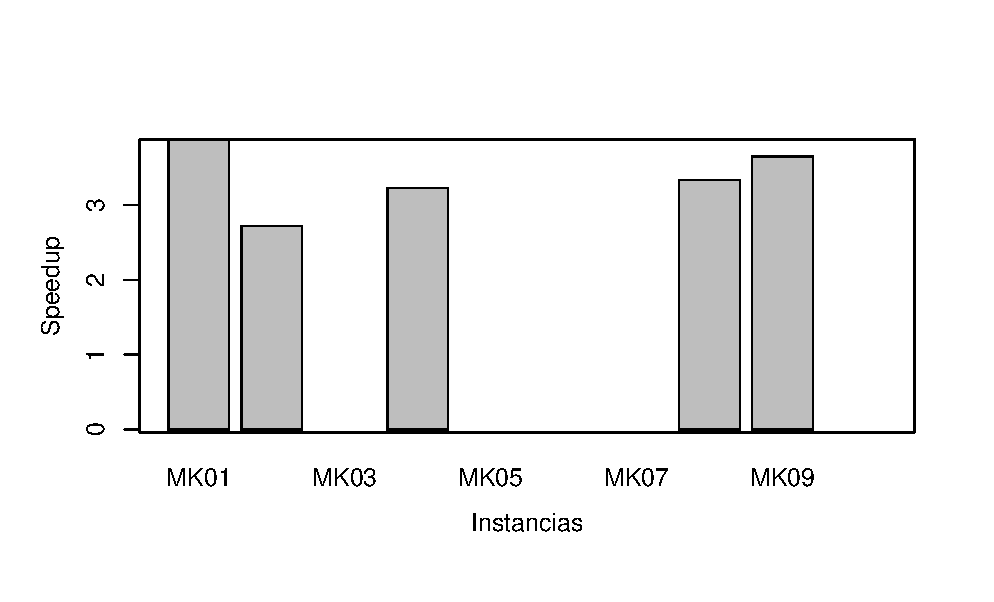
\includegraphics[trim={0 1cm 0 0.7cm},scale=0.7]{images/speedup.eps}
    \caption{\textit{Speedup} por instancia del FJSSP.}
    \label{fig:speedup}
\end{figure}

\section{Comparación de \textit{HDE} con la literatura}

Finalmente, se presenta una comparación de los valores de $C_{max}$ obtenidos por el \textit{HDE} con los alcanzados por varios algoritmos competitivos presentes en la literatura destinados a resolver el FJSSP. Esto permite determinar qué tan buena es la metaheurística presentada en este trabajo. En esta comparación, las metaheurísticas basadas en población para resolver el FJSSP consideradas fueron:

\begin{enumerate}[label=\textit{\roman*})]

\item hGA \cite{tang2011}: un algoritmo híbrido que combina la optimización por enjambre de partículas con un algoritmo genético.

\item BEDA \cite{Wang2012917}: un algoritmo de estimación de distribución basado en bi-poblaciones.

\item IACO \cite{WANG2017}: una optimización basada en colonia de hormigas.

\end{enumerate}

La Tabla \ref{tab:comparison} muestra que los valores de $C_{max}$ obtenidos por el \textit{HDE} son similares a los demás algoritmos para la mayoría de las diez instancias. Esta observación sugiere que el \textit{HDE} propuesto en este trabajo es un algoritmo competitivo para resolver el FJSSP. Las comparaciones con respecto al esfuerzo computacional son difíciles de llevar a cabo porque la mayoría de los trabajos no informan el número de evaluaciones. En consecuencia, la eficiencia relativa de los algoritmos comparados es difícil de contrastar para obtener comparaciones significativas.


\begin{table}[H]
\scriptsize
  \centering
  \caption{Comparación entre \textit{HDE} y metaheurísticas basadas en población de la literatura}
    \begin{tabular}{|l|c|c|c|c|c|c|c|c|c|c|}
    \hline
    \multicolumn{1}{|r}{} & \multicolumn{1}{|l}{MK01} & \multicolumn{1}{|l}{MK02} & \multicolumn{1}{|l}{MK03} & \multicolumn{1}{|l}{MK04} & \multicolumn{1}{|l}{MK05} & \multicolumn{1}{|l}{MK06} & \multicolumn{1}{|l}{MK07} & \multicolumn{1}{|l}{MK08} & \multicolumn{1}{|l}{MK09} & \multicolumn{1}{|l|}{MK10} \\
    \hline
    \textit{HDE}   & \textbf{40} & \textbf{26} & \textbf{204} & \textbf{60} & 173   & 61    & 140   & \textbf{523} & \textbf{307} & 224 \\
    hGA   & \textbf{40} & \textbf{26} & \textbf{204} & 62    & \textbf{172} & 65    & 140   & \textbf{523} & 310   & 214 \\
    BEDA  & \textbf{40} & \textbf{26} & \textbf{204} & \textbf{60} & \textbf{172} & 60    & \textbf{139} & \textbf{523} & \textbf{307} & 206 \\
    IACO  & \textbf{40} & \textbf{26} & \textbf{204} & \textbf{60} & 173   & 60    & 140   & \textbf{523} & \textbf{307} & 208 \\
\hline
    \end{tabular}%
  \label{tab:comparison}%
\end{table}%
    \chapter{Conclusión} 
En este trabajo se presentó un algoritmo \textit{DE} simple para resolver el FJSSP. Se hizo una revisión del material bibliográfico relacionado con técnicas metaheurísticas que ayudan a la comprensión de la tesis. Se describe una introducción a los algoritmos metaheurísticos, luego se presenta una de las posibles calificaciones de las metaheurísticas: en métodos basados en trayectoria y en métodos basados en poblaciones, y por último se explican distintos conceptos de diseños para paralelizar las metaheurísticas. Así también se hizo una revisión de los conceptos de la evolución diferencial, y se presenta el algoritmo propuesto por Storn \& Price, junto a sus 4 etapas: inicialización, mutación, recombinación y selección. Además se muestra el proceso iterativo del algoritmo \textit{DE} en un formato de pseudocódigo.


A continuación, se presenta una descripción del problema a tratar, el diseño de la representación y evaluación de soluciones utilizado, la decodificación de soluciones, el procedimiento de búsqueda local utilizado, la forma en que fue realizada la paralelización para acelerar el cálculo de \textit{DE} y la búsqueda local, y por último el pseudocódigo del algoritmo del \textit{HDE} para FJSSP, el cual sigue el esquema general de \textit{DE}, con la inclusión del proceso de búsqueda local. Además, se agrega como entrada la probabilidad de aplicar búsqueda local ($P_{BL}$), con el fin de permitir al investigador realizar cambios sobre el parámetro.


Finalmente, se describe el diseño experimental llevado a cabo para este trabajo donde fueron seleccionadas una amplia gama de instancias utilizadas en la literatura teniendo en cuenta su complejidad. Además, se analiza la calidad de los resultados considerando los valores de $ C_ {max} $ obtenidos para las distintas mejoras planteadas al algoritmo \textit{DE} descritas anteriormente para resolver las instancias de FJSSP. En primer lugar se estudia  el efecto de usar diferentes valores de $F$ y $Cr$ en el rendimiento del algoritmo, de valores bajos a altos (0.1, 0.5 y 0.9). Se observa que la combinación $F = 0.5 $ y $Cr = 0.9 $ supera a las demás desde el punto de vista de la calidad de los valores de $ C_ {max} $ obtenidos. 
Luego se analiza el impacto de la incorporación del proceso de búsqueda local a través del parámetro $P_{BL}$, donde fueron considerados tres valores diferentes: 0.1, 0.5 y 0.7 (de valores bajos a altos). Los resultados indican que el algoritmo \textit{HDE} con alta probabilidad de aplicar el procedimiento de búsqueda local, puede encontrar las mejores soluciones para el FJSSP. 
Posteriormente se evalúa el efecto en los tiempos al incorporar paralelismo a nivel de iteración. Los resultados muestran que el uso de la paralelización permite acelerar el tiempo de ejecución con respecto al \textit{HDE} secuencial sobre todas las instancias en un valor de 3 veces en promedio.
Por último, se presenta una comparación de los valores de $C_{max}$ obtenidos por el \textit{HDE} con los alcanzados por varios algoritmos competitivos presentes en la literatura destinados a resolver el FJSSP. Los valores de $C_{max}$ obtenidos por el \textit{HDE} son similares a los demás algoritmos para la mayoría de las diez instancias. Como consecuencia, el algoritmo \textit{HDE} propuesto en este trabajo ofrece buenas soluciones a este problema NP-duro de una manera eficiente.


En lo personal, me agradó la actitud de investigar y explorar en lo “desconocido” y en hacer cosas no imaginadas en un inicio, acudiendo al aprendizaje autodidacta con libros, papers, preguntando y solicitando consejos a mi directora y al grupo LISI, e incluso aprendiendo del modo ensayo/error en el proyecto desarrollado.


Aprendí que es muy diferente el estudio en las aulas, al de guiarse de un libro, y aún mas al de investigar académicamente, buscando nuevas propuestas para resolver problemas que no son triviales, expandiendo las fronteras del conocimiento, reflexionando críticamente y adaptándose a los formatos académicos.


Por último, reconocer que mi tesis no habría sido posible sin el apoyo de mi familia, amigos, y en especial a mi directora Carolina como así también a todo el grupo de investigación, que me sumaron a su equipo con una gran amabilidad y cordialidad desde el día uno. A todos ellos que me apoyaron, me dieron ánimos, conversamos, criticaron, etc, muchas gracias.

    
    

\begin{thebibliography}{9}
    \bibitem{haupt} 
    R. L. Haupt and S. E. Haupt
    \textit{Practical genetic algorithms.} 
    John Wiley \& Sons, 2004.

    \bibitem{Mitchell} 
    T. Mitchell.
    \textit{Machine Learning}. 
    McGraw Hill, 1997
    
    \bibitem{Brandimarte} 
    P. Brandimarte, “Routing and scheduling in a flexible job shop by tabu search,”
    \textit{Annals of Operations Research}, 
    vol. 41, p. 157183, 1993.

    \bibitem{GareyJohnson} 
    M. R. Garey, D. S. Johnson, R. Sethi, The complexity of flowshop and jobshop scheduling, Math. Oper. Res., vol. 1, no. 2, 1976, pp. 117–129.
    
    \bibitem{GareyJohnsonTheoryNP} 
    M. R. Garey, D. S. Johnson.
    \textit{Computers and Intractability: A Guide to the Theory of NP-Completeness}. 
    , 1979
    
    \bibitem{BlumRoli} 
    C. Blum, A. Roli, Metaheuristics in combinatorial optimization: Overview
    and conceptual comparison, ACM Computing Surveys 35 (3) (2003) 268–
    308
    
    \bibitem{YuanYuan} 
    Y. Yuan, H. Xu
    \textit{Flexible job shop scheduling using hybrid differential evolution algorithms}. 
    Computers \& Industrial Engineering, Volume 65, Issue 2, June 2013, Pages 246-260

    \bibitem{Apolloni} 
    J. M. Apolloni
    \textit{Propuesta de Metaheurísticas Híbridas para Mejorar el Análisis de Datos en Bioinformática (Ph.D. Tesis)}.
    Universidad Nacional de San Luis, 2017.
    
    \bibitem{Talbi} 
    E.-G. Talbi. A taxonomy of hybrid metaheuristics.
    \textit{Journal of Heuristics,}.
    8:541–564, 2002.
    
    \bibitem{openMP} 
    B. Chapman and G. Jost and R. van der Pas, 
    \textit{Using OpenMP: Portable Shared Memory Parallel Programming.}.
    MIT Press, 2007
    
    \bibitem{Ali} 
    M. Ali, W.A Zhu, Penalty function-based differential evolution algorithm for constrained global optimization, Comput. Optim. Appl., 54, 2013, pp. 707-739.
     
    \bibitem{Juang} 
    J.-G. Juang, S.-T. Yu, Disturbance encountered landing system design based on sliding mode control with evolutionary computation and cerebellar model articulation controller, Appl. Math. Model., 39, 2015, pp. 5862-5881.
     
    \bibitem{Yang} 
    Z. Yang, Q. Yu, W. Dong, X. Gu, W. Qiao, X. Liang, Structure control classification and optimization model of hollow carbon nanosphere core polymer particle based on improved differential evolution support vector machine, Appl. Math. Model., 37, 2013, pp. 7442-7451

    \bibitem{Garey} 
    M. R. Garey, D. S. Johnson, \& R. Sethi, The complexity of flowshop and jobshop scheduling.
    \textit{Mathematics of Operations Research,}.
     1, 117–129, 1976.
    
    \bibitem{albaMeta2005} 
     E. Alba,
    \textit{Parallel Metaheuristics: A New Class of Algorithms.}
     Wiley, 2005.
    
    \bibitem{bierwirth1995} 
    C. Bierwirth (1995). 
    A generalized permutation approach to job-shop scheduling with genetic algorithms. 
    Operations Research Spektrum. Vol. 17 (2). pp 87/92. 

    
    \bibitem{LuqueAlba} 
    G. Luque and E. Alba,
    \textit{Parallel Genetic Algorithms: Theory and Real World Ap-plications.}
    Springer Publishing Company, Incorporated, 2013.

    \bibitem{Goldberg} 
    D. E. Goldberg.
    \textit{Genetic Algorithms in Search, Optimization and Machine Learning}. 
    Addison-Wesley Longman Publishing Co., Inc., Boston, MA, USA, 1st edition, 1989.

    \bibitem{GarciaNietoAlba} 
    J. García-Nieto and E. Alba. Hybrid PSO6 for hard continuous optimization.
    \textit{Soft Computing}. 
    pages 1–19, 2014

    \bibitem{DorigoCaro} 
    M. Dorigo and G. Di Caro.
    \textit{New ideas in optimization}. 
    1999.
    
    \bibitem{Brownlee} 
    J. Brownlee.
    \textit{Clever Algorithms: Nature-inspired programming recipes.} 
    Jason Brownlee, 2011.
    
    \bibitem{Garcia-Nieto} 
    J. García-Nieto
    \textit{Emergent Optimization: Design and Applications in Telecomunications and Bioinformatics (Ph.D. Thesis).}
    University of Málaga, 2013.
    
    \bibitem{LaarhovenAarts} 
    P. J. M. Van Laarhoven and E. H. L. Aarts
    \textit{Simulated annealing.}
    Springer, 1987.

    \bibitem{LourencoStutzle} 
    H. R. Lourenço, O. C. Martin, and T. Stützle.
    \textit{Iterated local search.}
    Springer, 2003.
    
    \bibitem{HansenMladenovicBrimbergPerez} 
    P. Hansen, N. Mladenovic, J. Brimberg, and J. A. M. Pérez.
    \textit{Variable neighborhood search.} 
    In Handbook of Metaheuristics, pages 61–86. Springer, 2010.

    \bibitem{GendreauPotvin} 
    M. Gendreau and J-Y. Potvin
    \textit{Handbook of metaheuristics.}
    volume 2. Springer, 2010.

    \bibitem{PriceStornLampinen} 
    K. V. Price, R. Storn, and J. Lampinen
    \textit{Differential Evolution: A practical Approach to Global Optimization.}
    Springer-Verlag, London, UK, 2005.

    \bibitem{StornPrice} 
    R. Storn and K. V. Price. 
    Differential evolution: A simple and efficient adaptive scheme for global optimization over continuous spaces. 
     Technical report, TR95012-ICSI, 1995.

    \bibitem{StornPrice2} 
    R. Storn, K. Price Differential evolution—a simple and efficient heuristic for global optimization over continuous spaces. 
    \textit{Journal of Global Optimization.}
    1997;11(4):341–359. 
    
    \bibitem{Colorni} 
    A. Colorni, M. Dorigo, V. Maniezzo Distributed optimization by ant colonies. Proceedings of the 1st European Conference on Artificial Life; 1991; Paris, France. pp. 134–142.
    
    \bibitem{StornPriceConference} 
    R. Storn and K. V. Price. 
    Minimizing the real functions of the ICEC’96 contest by differential evolution. 
    In \textit{International Conference on Evolutionary Computation},pages 842–844, 1996.

    \bibitem{KennedyEberhartShi} 
    J. Kennedy, R. Eberhart, and Y. Shi.
    \textit{Swarm Intelligence}. 
    Morgan Kaufmann, San Francisco, CA, 2001.
    
    \bibitem{Eberhart} 
    R. C. Eberhart, J. Kennedy New optimizer using particle swarm theory. Proceedings of the 6th International Symposium on Micro Machine and Human Science; October 1995. pp. 39–43.
    
    \bibitem{BlumLi} 
    C. Blum and X. Li.
    \textit{Swarm intelligence in optimization}. 
    Springer, 2008.

    \bibitem{Dasgupta} 
    D. Dasgupta.
    \textit{Artificial immune systems and their applications}. 
    Springer Publishing Company, Incorporated, 2014.  
    
    
    \bibitem{KirkpatrickVecchi} 
    S. Kirkpatrick, M. P. Vecchi, et al. 
    \textit{Optimization by simmulated annealing.}
    Science, 220(4598):671–680, 1983.  

    \bibitem{Cerny} 
    V. Cerny. Thermodynamical approach to the traveling salesman problem: An 
    efficient simulation algorithm. 
    \textit{Journal of optimization theory and applications}
    , 45(1):41–51, 1985.  
    
    \bibitem{MetropolisRosenbluth} 
    N. Metropolis, A. Rosenbluth, M. Rosenbluth, A. Teller, and E. Teller. Equation of state
    calculations by fast computing machines.
    \textit{Journal of Chemical Physics,}. 
    21:1087–1092, 1953.  
    
    \bibitem{HansenMladenovic} 
    P. Hansen and N. Mladenovic. Variable neighborhood search: Principles and applications.
    \textit{European Journal of Operational Research, }. 
    130(3):449–467, 2001.  
    
    \bibitem{QinSuganthan} 
    A.K. Qin and P.N. Suganthan. Self-adaptive differential evolution algorithm for numerical optimization. In
    \textit{Proceedings of the 2005 IEEE Congress on Evolutionary Computation }. 
    , volume 2, pages 1785–1791, 2005.      
    
    \bibitem{BrestGreinerBoskovicMernik} 
    J. Brest, S. Greiner, B. Boskovic, M. Mernik, and V. Zumer. Self-adapting control
    parameters in differential evolution: A comparative study on numerical benchmark
    problems.
    \textit{s. IEEE Transactions on Evolutionary Computation, }. 
    10(6):646–657, 2006.   
    
    \bibitem{Holland} 
     J. H. Holland. Outline for a logical theory of adaptive systems.
    \textit{Journal of the ACM}. 
    3:297–314, 1962.
    
    \bibitem{Holland2} 
     J. H. Holland.
    \textit{Adaptation in Natural and Artificial Systems}. 
    University of Michigan Press, Ann Arbor, MI, 1975.

    \bibitem{Holland3} 
    J. H. Holland 
    \textit{Adaptation in Natural and Artificial Systems: An Introductory Analysis with Applications to Biology, Control, and Artificial Intelligence}. 
    MIT Press; 1992.


    \bibitem{Rechenberg} 
    I. Rechenberg.
    Cybernetic solution path of an experimental problem. 
    Technical Report, Royal Aircraft Establishment Library Translation No. 1112, Farnborough, UK, 1965.

    \bibitem{Rechenberg2} 
    I. Rechenberg.
    \textit{Evolutionstrategie: Optimierung technischer systeme nach prinzipien der biologischen evolution.}. 
    Frommann-Holzboog, 1973.

    \bibitem{Schott} 
    J. R. Schott.
    Fault tolerant design using single and multicriteria genetic algorithm optimization. 
    PhD thesis, Department of Aeronautics and Astronautics, Massachusetts Institute of Technology, Cambridge, MA, 1995.

    \bibitem{Schwefel} 
     H-P. Schwefel.
    Kybernetische evolution als strategie der experimentellen forschung in der stromungstechnik. 
    Technical report, Diplomarbeit Hermann Fottinger Institut fur Stromungstechnik, Technische universit at, Berlin, Germany, 1965.

    \bibitem{Fogel} 
    L. J. Fogel. Toward inductive inference automata. In
    \textit{Proceedings of the International Federation for Information Processing Congress}. 
     Munich, 1962, pp. 395–399.

    \bibitem{FogelOwens} 
    L. J. Fogel, A. J. Owens, and M. J. Walsh.
    \textit{Artificial Intelligence Through Simulated Evolution.}. 
    Wiley, 1966.

    \bibitem{Koza} 
    J. R. Koza
    \textit{Genetic Programming.}. 
    MIT Press, Cambridge, MA, 1992.

    \bibitem{BackFogelMichalewicz} 
    T. Back, D. B. Fogel, and Z. Michalewicz, editors.
    \textit{Handbook of Evolutionary Computation.}. 
    Oxford University Press, 1997.
    
    \bibitem{CorneDorigoDasguptaMoscato} 
    D. Corne, M. Dorigo, F. Glover, D. Dasgupta, P. Moscato, R. Poli, and K. V. Price.
    \textit{New ideas in optimization.}. 
    McGraw-Hill Ltd., UK, 1999.
    
    \bibitem{Moscato} 
     P. C3P Report. 826. Caltech Concurrent Computation Program; 1989. On evolution, search, optimization, genetic algorithms and martial arts: towards memetic algorithms.  
    
    \bibitem{DorigoBirattari} 
    M. Dorigo, M. Birattari, and T. Stützle. Ant colony optimization.
    \textit{Computational Intelligence Magazine}. 
    IEEE, 1(4):28–39, 2006.

    \bibitem{KarabogaBasturk} 
    D. Karaboga and B. Basturk. A powerful and efficient algorithm for numerical function optimization: artificial bee colony (abc) algorithm. 
    \textit{Journal of Global Optimization, }. 
    39(3):459–471, 2007.
    
    \bibitem{Rudolph} 
    G. Rudolph. Convergence of evolutionary algorithms in general search spaces.
    \textit{In Proceedings of the Third IEEE Conference on Evolutionary Computation,}
    1996.
    
    \bibitem{Gnanavel} 
    A. Gnanavel Babu, J. Jerald, A. Noorul Haq , V. Muthu Luxmi, T. Vigneswaralu, Scheduling of machines and automated guided vehicles in FMS using differential evolution, Int. J. Prod. Res., 48 ,2010, pp. 4683-4699.
    
    \bibitem{Melo} 
    V.V. De Melo, G.L. Carosio, Investigating multi-view differential evolution for solving constrained engineering design problems, Expert Syst. Appl., 40, 2013, pp. 3370-3377.
    
    \bibitem{Karaboga} 
    D. Karaboga. 
    An idea based on honey bee swarm for numerical optimization.. 
    Technical Report TR06, Erciyes University, 2005.
    
    \bibitem{CastroTimmis} 
    L. N. De Castro and J. Timmis.
    \textit{Artificial immune systems: a new computational intelligence approach.}. 
    Springer Science \& Business Media, 2002.
    
    \bibitem{TalbiLibro} 
    E-G Talbi
    \textit{Metaheuristics: from design to implementation}. 
    Wiley, Hoboken, 2009.
    
    \bibitem{MinettiSalto} 
    C. Bermudez, G. Minetti and C. Salto, 
    \textit{Improving Artificial Bee Colony Algorithm with Evolutionary Operators} Facultad de Ingeniería, Universidad Nacional de La Pampa, CONICET, Argentina, 2017.
    
    \bibitem{tang2011} 
    J. Tang, G. Zhang, B. Lin and B. Zhang,
    ``A hybrid algorithm for flexible job-shop scheduling problem``, 
    \textit{Procedia Engineering}, vol 15, pp. 3678 - 3683, 2011.
    
    \bibitem{Wang2012917} 
    L. Wang, S. Wang, Y. Xu, G. Zhou and M. Liu, 
    ``A bi-population based estimation of distribution algorithm for the flexible job-shop scheduling problem``, 
    \textit{Computers \& Industrial Engineering }, vol 62, no. 4, pp. 917 - 926, 2012.

    \bibitem{WANG2017} 
    L. Wang, J. Cai, M. Li and Z. Liu, 
    ``Flexible job-shop scheduling problem using an improved ant colony optimization``,
    \textit{Scientific Programming}, pp. 1 - 11, 2017.
\end{thebibliography}


\end{document}
